\documentclass[UTF8,12pt]{article}
\usepackage{ctex}
\usepackage{indentfirst}
\usepackage{color}
\usepackage{hyperref}
\usepackage{graphicx}
\usepackage{subfigure}
\usepackage{pdfpages}
\usepackage{listings}
\hypersetup{
    hidelinks,
	colorlinks=true,
	allcolors=black,
	pdfstartview=Fit,
	breaklinks=true
}

\definecolor{dkgreen}{rgb}{0,0.6,0}
\definecolor{gray}{rgb}{0.5,0.5,0.5}
\definecolor{mauve}{rgb}{0.58,0,0.82}

\lstset{ %
  language=Octave,                % the language of the code
  basicstyle=\footnotesize,           % the size of the fonts that are used for the code
  numbers=left,                   % where to put the line-numbers
  numberstyle=\tiny\color{gray},  % the style that is used for the line-numbers
  stepnumber=2,                   % the step between two line-numbers. If it's 1, each line 
                                  % will be numbered
  numbersep=5pt,                  % how far the line-numbers are from the code
  backgroundcolor=\color{white},      % choose the background color. You must add \usepackage{color}
  showspaces=false,               % show spaces adding particular underscores
  showstringspaces=false,         % underline spaces within strings
  showtabs=false,                 % show tabs within strings adding particular underscores
  frame=single,                   % adds a frame around the code
  rulecolor=\color{black},        % if not set, the frame-color may be changed on line-breaks within not-black text (e.g. commens (green here))
  tabsize=2,                      % sets default tabsize to 2 spaces
  captionpos=b,                   % sets the caption-position to bottom
  breaklines=true,                % sets automatic line breaking
  breakatwhitespace=false,        % sets if automatic breaks should only happen at whitespace
  title=\lstname,                   % show the filename of files included with \lstinputlisting;
                                  % also try caption instead of title
  keywordstyle=\color{blue},          % keyword style
  commentstyle=\color{dkgreen},       % comment style
  stringstyle=\color{mauve},         % string literal style
  escapeinside={\%*}{*)},            % if you want to add LaTeX within your code
  morekeywords={*,...}               % if you want to add more keywords to the set
}


\setlength{\parindent}{2em}

\begin{document}



\begin{center}
    \tableofcontents
\end{center}
\newpage

\section{实验目标与基本要求}
\subsection{实验目标}
开发网络爬虫在东方财富、新浪财经或者纳斯达克等财经网站上爬取一只股票的每天的开盘价,收盘价,最高价,最低价等信息,并存储在数据库中,并开发GUI应用可视化。

\subsection{基本要求}
(1) 掌握网络爬虫的开发方法;

(2) 掌握Python开发数据库的GUI界面;

(3) 掌握Matplotlib绘制股票的K线图;

\section{主要知识点、重点与难点}
\subsection{主要知识点}
1.	网络爬虫的基本知识;

2.	利用正则表达式对网页信息提取;

3.	数据库的访问和表中的数据操作;

4.	Matplotlib库的使用

\subsection{重点}
1.	网络爬虫框架的使用;

2.	正则表达式的使用;

3.	数据库存储数据

\subsection{难点}
1.	利用正则表达式根据网页中的信息组织方式提取数据;

2.	K线图的展现。

\section{实验过程设计}
1)	在互联网中寻找可以提取数据的网站;

2)	构造网络爬虫框架以及正则表达式;

3)	设计数据库表,建立数据库,将获取的数据存储到数据库中;

4)	设计数据库访问语句,可以以表格的形式展现数据;

5)	可以将一只股票30天的数据用K线图展现。

\section{主要实现过程}

\subsection{爬虫准备}

\subsubsection{确定网站:搜狐股票}
根据实验要求,本次实验不限制爬取对象,由于Nasdaq为国外网站,访问时不能直接出现数据,因此本次实验选取了搜狐证券进行爬虫操作。

网址:
\href{https://q.stock.sohu.com/cn/}{https://q.stock.sohu.com/cn/}

\begin{figure}[htbp]
    \centering
    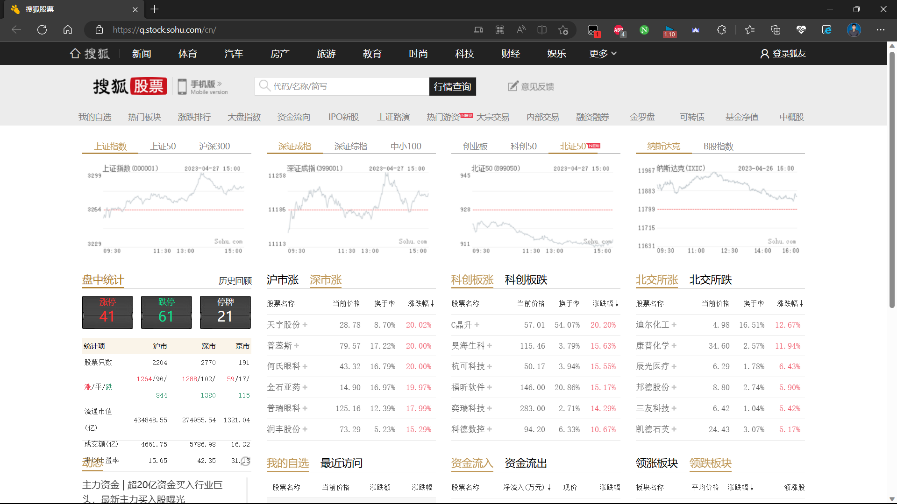
\includegraphics[width=0.5\textwidth]{img/1.png}
    \caption{搜狐股票网站}
\end{figure}

\newpage

对于某只特定的股票,通过分析网址,只需要在上述的url+该股票代码+ /lshq.shtml,就可以进入股票历史数据界面,以贵州茅台为例:
\begin{figure}[htbp]
    \centering
    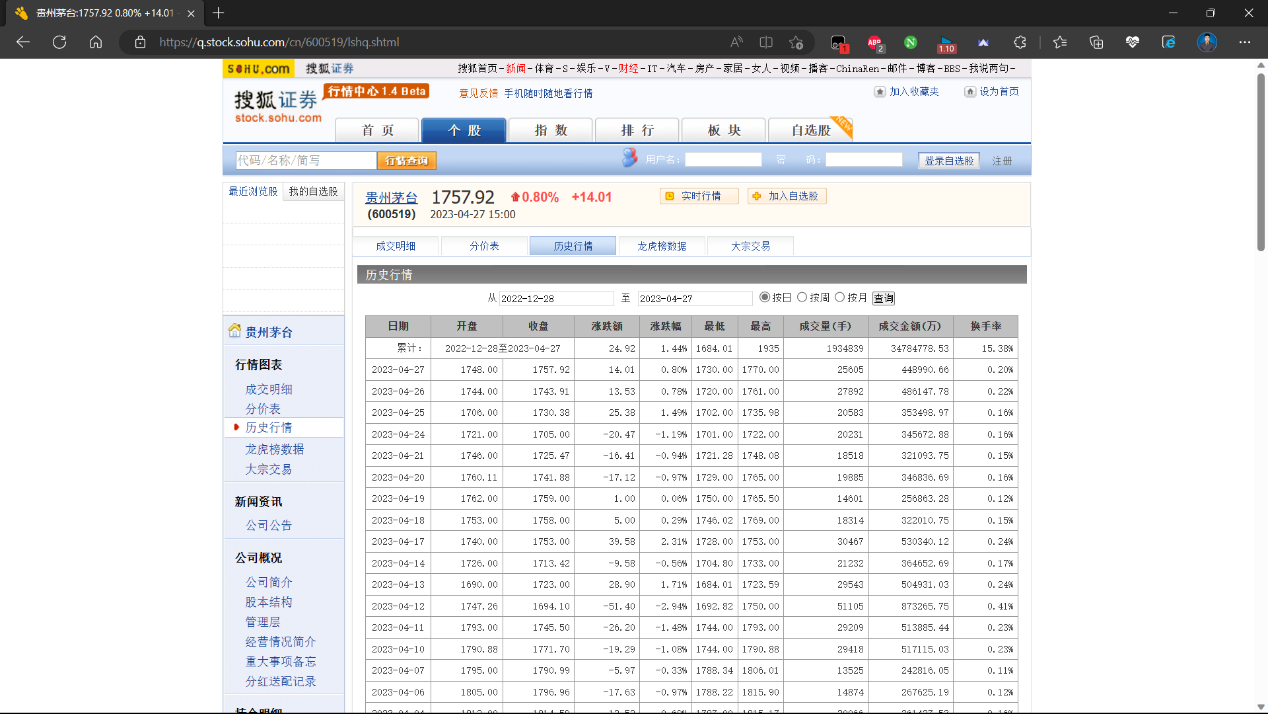
\includegraphics[width=0.8\textwidth]{img/2.png}
    \caption{贵州茅台股票历史数据}
\end{figure}

\subsubsection{查看爬取元素的代码}
进入网站开发者模式(按下F12)查看网页的源代码,点击元素,鼠标指向页面中的元素,通过这个工具确定需要爬取的部分的源代码
\begin{figure}[htbp]
    \centering
    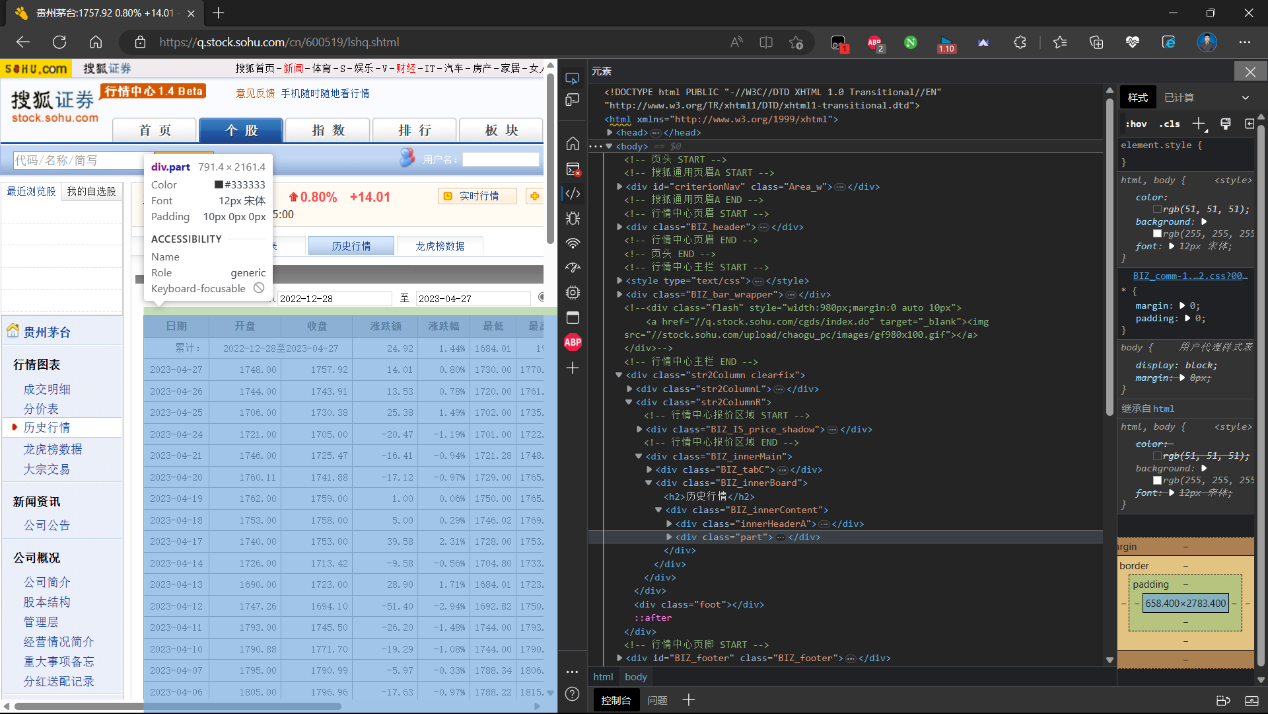
\includegraphics[width=0.6\textwidth]{img/3.png}
    \caption{查看源代码}
\end{figure}

通过元素选取确定了数据表格的
$$class='tableQ'$$
$$id='BIZ\_hq\_historySearch'$$

\begin{figure}[htbp]
    \centering
    \subfigure[确定数据表格相关属性]{
        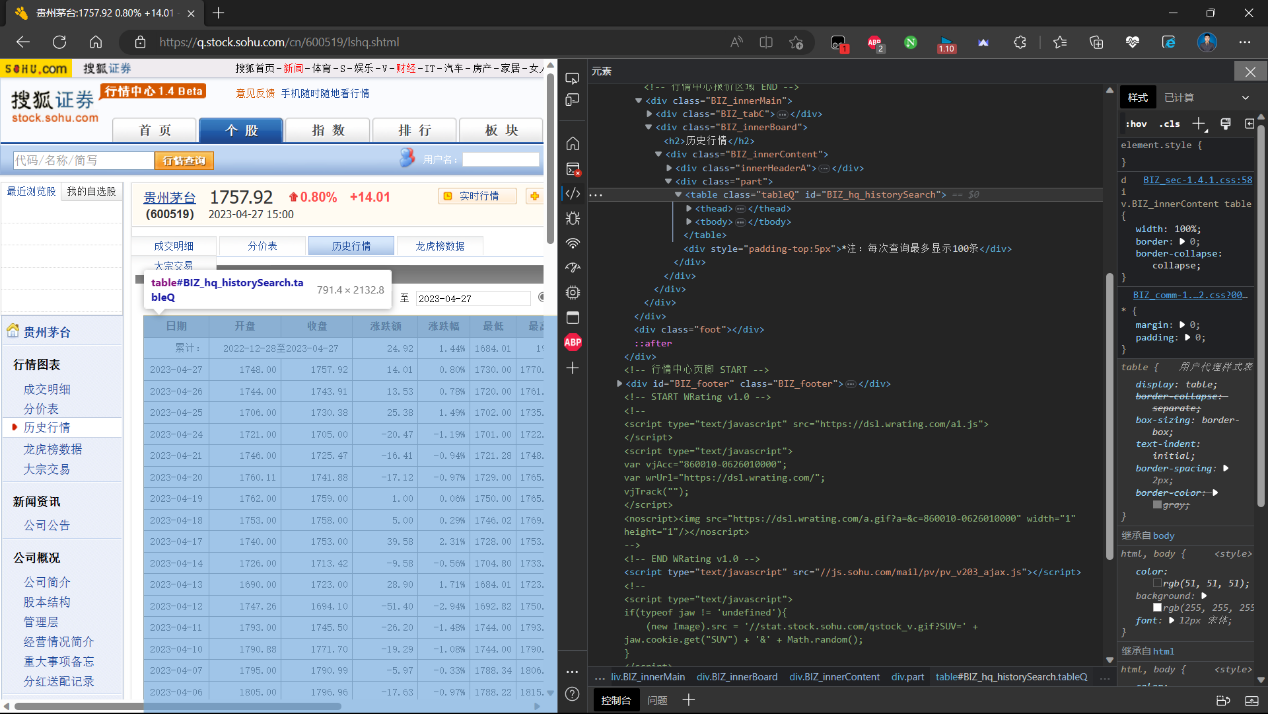
\includegraphics[scale=0.5]{img/4.png} \label{1}
    }
    \subfigure[定位表格]{
        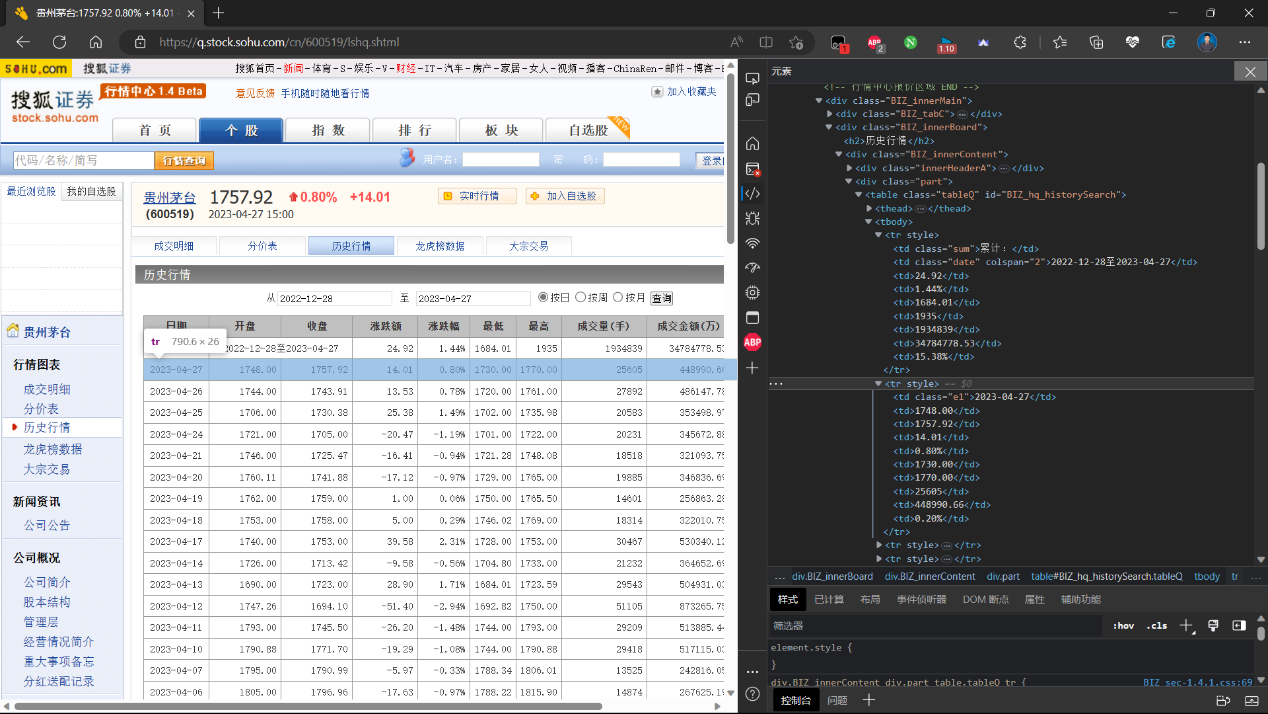
\includegraphics[scale=0.5]{img/5.png} \label{2}
    }
    \caption{源代码审查}
\end{figure}

\newpage

\subsubsection{精准确定爬取元素}
观察页面布局可以发现表格体的第一行是累计,而累计并不是本实验所需要的数据,因此确定爬取数据从第二行开始

\begin{figure}[htbp]
    \centering
    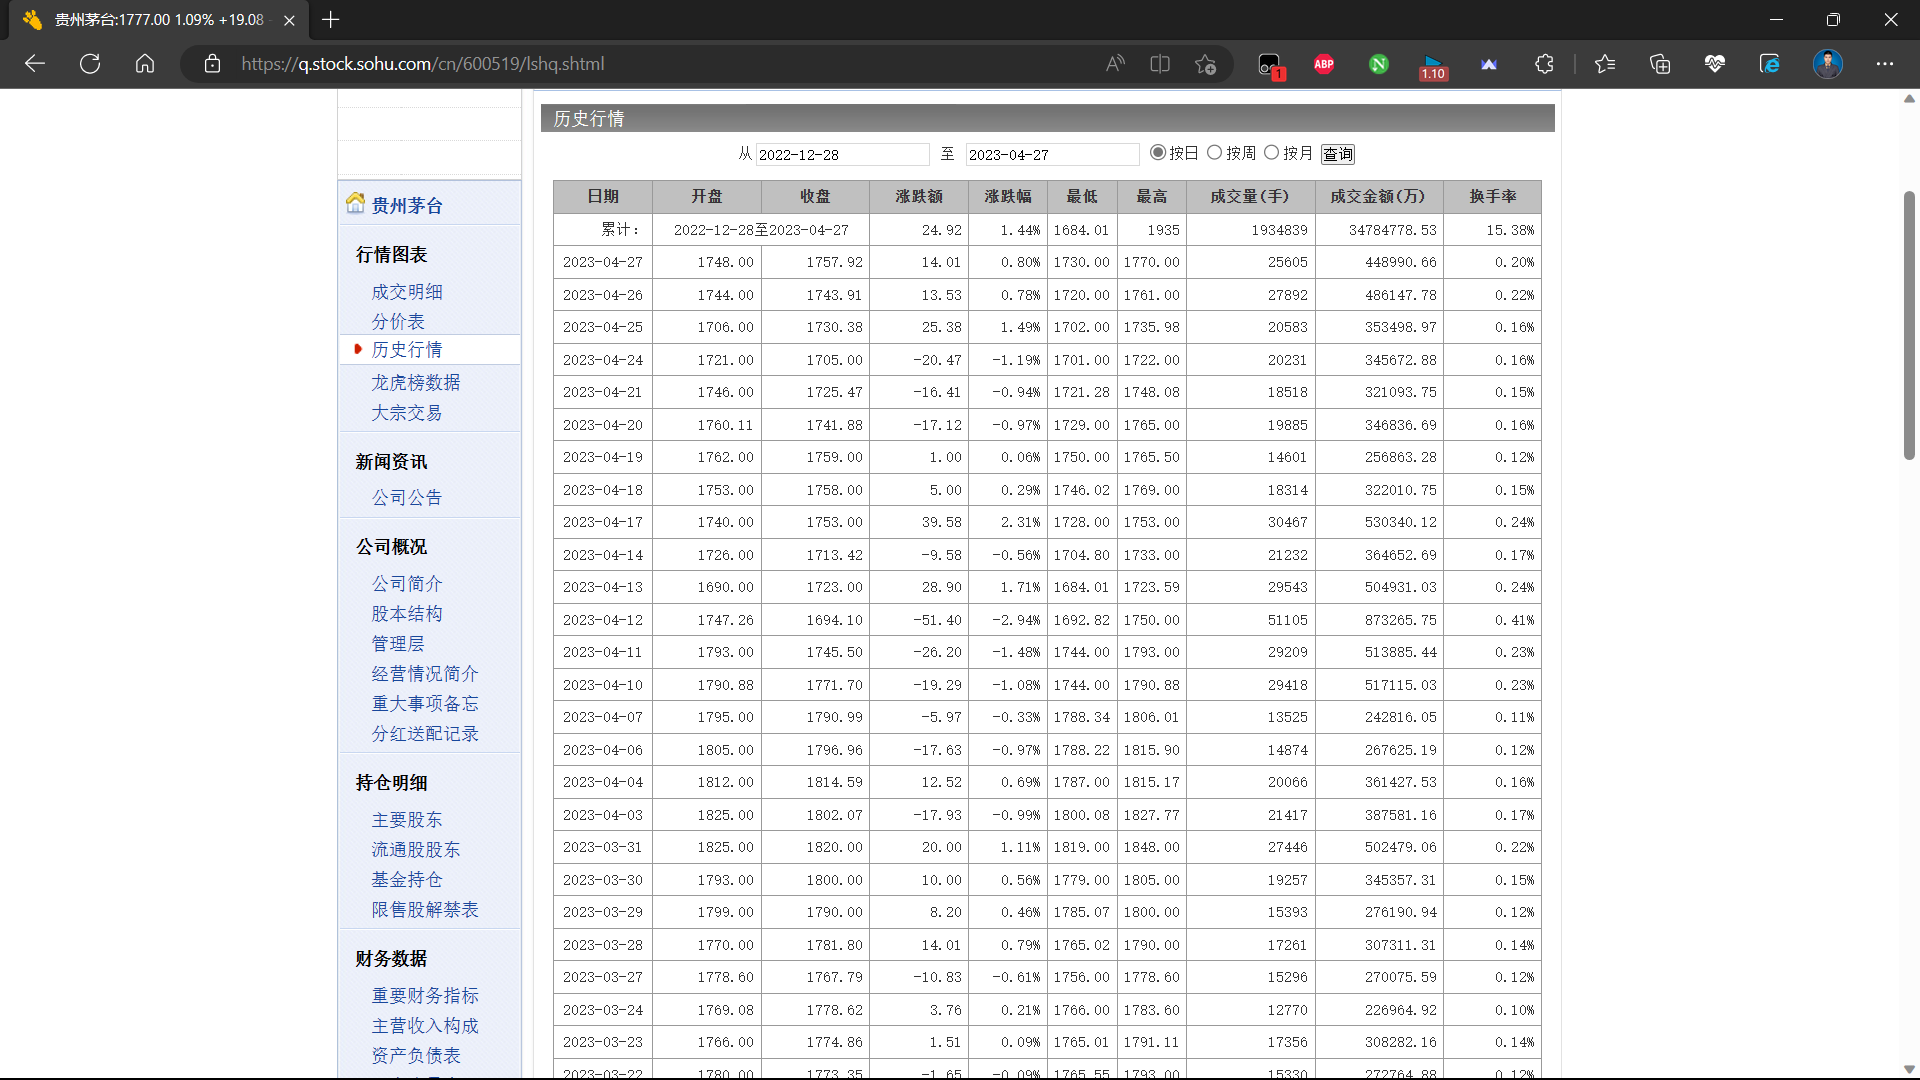
\includegraphics[width=0.6\textwidth]{img/6.png}
    \caption{分析表格元素}
\end{figure}

\subsection{获取HTML代码}
\subsubsection{伪装用户}
使用request库对网页源代码进行爬取,分析得知,网站的历史行情数据都是动态数据,无法通过静态方式爬取,因此使用selenium库进行数据爬取

\begin{lstlisting}[title=调用selenium库, frame=shadowbox]
from selenium import webdriver
from selenium.webdriver.common.by import By
driver = webdriver.Chrome()
driver.get('http://q.stock.sohu.com/cn/'+stack_code+'/lshq.shtml')
time.sleep(5)
\end{lstlisting}

\subsubsection{使用findelement爬取相关表格}
在尝试这种方法之前,曾经尝试使用beautifulsoup库通过类定位爬取数据表格,但是最终失败了,改变策略使用findelement,并调用By.XPATH,通过xpath来定位数据表格的相关属性并爬取,在确定xpath的时候,使用了正则表达式来定位,在chrome的开发者模式下,对网页元素分析可以直接获得xpath
\begin{figure}[htbp]
    \centering
    
\includegraphics[width=0.8\textwidth]{img/7.png}
    \caption{获取元素xpath}
\end{figure}

将获得的xpath放入findelement函数,然后将爬取的数据存放在kv字典中,再通过循环结构重复每一行的爬取操作。

\begin{lstlisting}[frame=shadowbox]
    f=open("data.txt","w",encoding="utf-8")

    for i in range(2, 81):
        kv={}
        try:
            kv["日期"] = driver.find_element(By.XPATH,'//*[@id="BIZ_hq_historySearch"]/tbody/tr['+str(i)+']/td[1]').text
\end{lstlisting}
    
\begin{lstlisting}[title=findelement数据爬取,frame=shadowbox]
            kv["开盘价"] = driver.find_element(By.XPATH,'//*[@id="BIZ_hq_historySearch"]/tbody/tr['+str(i)+']/td[2]').text
            kv["最高价"] = driver.find_element(By.XPATH,'//*[@id="BIZ_hq_historySearch"]/tbody/tr['+str(i)+']/td[7]').text
            kv["最低价"] = driver.find_element(By.XPATH,'//*[@id="BIZ_hq_historySearch"]/tbody/tr['+str(i)+']/td[6]').text
            kv["收盘价"] = driver.find_element(By.XPATH,'//*[@id="BIZ_hq_historySearch"]/tbody/tr['+str(i)+']/td[3]').text
            kv["成交量"] = driver.find_element(By.XPATH,'//*[@id="BIZ_hq_historySearch"]/tbody/tr['+str(i)+']/td[8]').text
            print("complete")
        except:
            print("找不到元素")
            continue
        month_data.append(kv)
        to_write = json.dumps(kv,ensure_ascii=False)
        f.write(to_write)
    f.close()
\end{lstlisting}

由于后续有绘制K线图的需求,在数据方面,本实验只需要存储日期、开盘价、最高价、最低价和收盘价等数据,此外再加入成交量,至此爬取数据部分完毕。

\subsection{数据存储}
本实验使用MySQL数据库,数据存储实现直接调用pymysql库,并定义存储函数,在存储函数中实现创建数据库、创建表、插入数据等操作.

\subsubsection{创建数据库、表}
在python中,通过pymysql库能够实现与数据库连接,并使用python代码实现sql语句的调用。

先在存储函数中生成游标对象,使用游标对象实现数据库的相关操作

\begin{lstlisting}[title=生成游标对象,frame=shadowbox]
    cursor = my_database.cursor()
\end{lstlisting}

然后通过游标对象创建数据库
\begin{lstlisting}[title=创建数据库,frame=shadowbox]
    sql_createDataBase = "create database if not exists stockData"
    cursor.execute(sql_createDataBase)
    sql_useDataBase = "USE stockData"
\end{lstlisting}

对数据表进行设计
\begin{lstlisting}[title=数据表的设计,frame=shadowbox]
    create table if not exists data
    (
        date DATE,
        opening_price float,
        closing_price float,
        highest float,
        lowest float
    )
\end{lstlisting}

\newpage

通过游标对象创建表
\begin{lstlisting}[title=创建表,frame=shadowbox]
    cursor.execute(sql_useDataBase)
    sql_createTable = '''
    create table if not exists data
    (
        date DATE,
        opening_price float,            closing_price float,
        highest float,
        lowest float
    )
    '''
    cursor.execute(sql_createTable)
\end{lstlisting}
    
\subsubsection{数据插入数据库}

先写出sql的数据插入语句
\begin{lstlisting}[title=sql数据插入语句]
    Insert into data values('date','opening_price','closing_price','highest','lowest')
\end{lstlisting}

对于本实验数据库的数据表,只存储后续需要画K线图的日期、开盘价、收盘价、最高价、最低价,在定义存储函数的时候,将待存储的数据以字典类型作为变量存入数据库中,在字典列表中取出数据,使用for循环将数据拆分,分别传入数据

\begin{lstlisting}[title=数据插入数据库,frame=shadowbox]
    for item in data:
        sql_Insert = '''Insert into data values('{0}',{1},{2},{3},{4})'''.format(item['日期'], item['开盘价'], item['收盘价'], item['最高价'], item['最低价'])
        cursor.execute(sql_Insert)
\end{lstlisting}

至此数据库、表创建完成,存储函数实现

\subsubsection{txt文件的生成}
在findelement数据爬取代码段中,同时实现了将待存储数据转换成json数据格式并写入data.txt文件中,在后续的数据分析操作中便于python其他库读取

\begin{lstlisting}[title=txt文件存储,frame=shadowbox]
    f=open("data.txt","w",encoding="utf-8")

    for i in range(2, 81):
        kv={}
        try:
            ...
        except:
            ...
        month_data.append(kv)
        to_write = json.dumps(kv,ensure_ascii=False)
        f.write(to_write)
    f.close()
\end{lstlisting}

\subsection{创建图形化界面}
\subsubsection{设计图形化界面}
本实验使用wxpython库创建GUI界面。

设计了一个简单的界面:

界面的左侧是预留空间,用来打印输出某只股票的历史行情数据表格;

界面的右侧有一个文本框,用来输入股票代码;

文本框下方有三个按钮,分别是“查询K图”、“更新”和“查看表格”,实现功能如下:

查询K图:点击后,打开一个html文件,内部存有已经绘制好的K线图;

更新:先在文本框最终输入想要查询的股票代码,点击更新后,爬取数据并存入数据库,同时生成一个xlsx表格,用来正确性验证;

查看表格:点击后,在左侧预留空间打印输出某只股票的历史行情数据表格。

\begin{figure}[htbp]
    \centering
    
\includegraphics[width=0.8\textwidth]{img/8.png}
    \caption{图形化界面}
\end{figure}

\subsubsection{构建MyFrame类}
对于MyFrame类的设计,首先在类的初始化函数中,定义了一个panel,用来存放界面的各个组件,然后在panel中定义了一个文本框,用来输入股票代码,文本框下方有三个按钮,分别是“查询K图”、“更新”和“查看表格”,代码实现如下:

\begin{lstlisting}
class MyFrame(wx.Frame):
    data = []
    column_names = []
    stock_Code = ""

    def __init__(self, data, column_names):
        super().__init__(parent=None, title="股票数据显示界面", size=(600, 600))
        self.data = data
        self.column_names = column_names
        self.Centre()
        panel = wx.Panel(parent=self)
        # self.message1 = wx.StaticText()
        # self.message1.SetLabelText("请输入股票代码")
        # self.message1.SetPosition((400,370))
        self.number = wx.TextCtrl(panel, pos=(450, 370))
        query_button = wx.Button(parent=panel, id=1, label='查询K图', pos=(450, 400))
        post = wx.Button(parent=panel, id=2, label='更新', pos=(450, 435))
        show = wx.Button(parent=panel, id=3, label='查看表格', pos=(450, 470))
        self.Bind(wx.EVT_BUTTON, self.on_click, query_button)
        self.Bind(wx.EVT_BUTTON, self.on_click, post)
        self.Bind(wx.EVT_BUTTON, self.on_click, show)
        # self.Bind(wx.EVT_TEXT, self.EvtText)
        # 建立表格
\end{lstlisting}

\begin{lstlisting}
    def generate_xlsx(self):
        self.grid = self.CreateGrid(self)
        self.Bind(wx.grid.EVT_GRID_LABEL_LEFT_CLICK, self.OnLabelLeftClick)

    def on_click(self, event):
        event_id = event.GetId()
        print(event_id)
        if event_id == 1:
            print("查询K图")
            webbrowser.open('K图.html')
        elif event_id == 2:
            self.stock_Code = self.number.GetValue()
            print(self.number.GetValue())
            update_xlsx(self, self.stock_Code)
        elif event_id == 3:
            self.generate_xlsx()

    def OnLabelLeftClick(self, event):
        print("RowIdx:{0}".format(event.GetRow()))
        print("ColIdx:{0}".format(event.GetCol()))
        print(self.data[event.GetRow()])
        event.Skip()

    def CreateGrid(self, parent):
        grid = wx.grid.Grid(parent)
        grid.CreateGrid(len(self.data), len(self.data[0]))

        for row in range(len(self.data)):
            for col in range(len(self.data[row])):
                grid.SetColLabelValue(col, self.column_names[col])
\end{lstlisting}

\newpage

\begin{lstlisting}[title=MyFrame的构建,frame=shadowbox]
                grid.SetCellValue(row, col, self.data[row][col])
         # 设置行和列自定调整
        grid.AutoSize()

        return grid
\end{lstlisting}

\subsubsection{构建窗口对象}
在窗口对象中,首先调用了MyFrame类的构造函数,然后调用了Show()方法显示窗口,实现代码如下:

\begin{lstlisting}[title=构建窗口对象,frame=shadowbox]
class App(wx.App):
    data = []
    column_names = []

    def show(self):
        frame = MyFrame(self.data, self.column_names)
        frame.Show()
        return True
\end{lstlisting}

\subsubsection{按钮功能的实现}
界面一共有三个按钮,分别是“查询K图”、“更新”和“查看表格”,实现功能如下:

查询K图:点击后,打开一个html文件,内部存有已经绘制好的K线图;

更新:先在文本框最终输入想要查询的股票代码,点击更新后,爬取数据并存入数据库,同时生成一个xlsx表格,用来正确性验证;

查看表格:点击后,在左侧预留空间打印输出某只股票的历史行情数据表格。

代码实现如下:
\begin{lstlisting}[title=按钮功能实现,frame=shadowbox]
def on_click(self, event):
    event_id = event.GetId()
    print(event_id)
    if event_id == 1:
        print("查询K图")
        webbrowser.open('K图.html')
    elif event_id == 2:
        self.stock_Code = self.number.GetValue()
        print(self.number.GetValue())
        update_xlsx(self, self.stock_Code)
    elif event_id == 3:
        self.generate_xlsx()
\end{lstlisting}

\subsubsection{grid构建}
在grid构建中,首先调用了CreateGrid()方法,然后调用了AutoSize()方法,实现代码如下:

\begin{lstlisting}[title=grid构建,frame=shadowbox]
def CreateGrid(self, parent):
    grid = wx.grid.Grid(parent)
    grid.CreateGrid(len(self.data), len(self.data[0]))

    for row in range(len(self.data)):
        for col in range(len(self.data[row])):
            grid.SetColLabelValue(col, self.column_names[col])
            grid.SetCellValue(row, col, self.data[row][col])
    # 设置行和列自定调整
    grid.AutoSize()
\end{lstlisting}

\subsection{数据处理及可视化}
本实验中,主要的数据处理及可视化项目就是K线图的绘制,在绘制前需要做相应的数据处理

\subsubsection{数据处理}
本项目的数据处理主要是将绘制K线图所需的五个对应数据分别放进五个列表中。

\begin{lstlisting}[title=数据处理,title=shadowbox]
def data_Pretreatment(month_data):
    for data in month_data:
        my_date = data.get("日期")
        my_open = data.get("开盘价")
        my_close = data.get("收盘价")
        my_high = data.get("最高价")
        my_low = data.get("最低价")
        date.append(my_date)
        opening_price.append(my_open)
        closing_price.append(my_close)
        highest.append(my_high)
        lowest.append(my_low)
\end{lstlisting}

\subsubsection{K线图的绘制}
本次实验的K线图绘制并没有使用Matplotlib库,而是通过pyecharts库来实现的,pyecharts是一个用于生成Echarts图表的类库,它提供了一种使用Python构建Echarts图表的简单方法。pyecharts支持Python2.7+和Python3.4+,并且兼容多种操作系统。pyecharts的安装也非常简单,只需要在命令行中输入pip install pyecharts即可。

在pyecharts库中,有Kline类可以直接调用,只需要整合好一组数据输入Kline的一个实例对象就可以生成K线图

实现代码如下:
\begin{lstlisting}[title=K线图绘制,frame=shadowbox]
def draw_K():
    kline = Kline().set_global_opts(title_opts=opts.TitleOpts(title="K线图"))
    v1 = []
    size = len(opening_price)  # 有多少条数据(多少天)
    for i in range(size-1, 0, -1):
        tmp = [opening_price[i], closing_price[i], lowest[i], highest[i]]
        v1.append(tmp)  # 整合好一组数据存入v1中
    # print(v1)

    kline.add_yaxis(series_name="日K", y_axis=v1)
    kline.add_xaxis([s for s in date])
    kline.render("K图.html")
\end{lstlisting}

K线图绘制函数的最终返回一个绘有月K线图的html文件,在“查询K图”的按钮事件中,使用webbrowser.open通过浏览器打开html文件

至此,本实验的主要实现过程基本阐述完毕

\section{效果展示}
效果展示分别展示控制台输出情况和界面的运行情况

\subsection{开始运行展示}
在pycharm代码界面,由于预设了股票代码300117,在右键点击运行后,会首先爬取300117的相关数据,并生成对应的图、数据库、txt文件

\begin{figure}[htbp]
	\centering
	\begin{minipage}{0.49\linewidth}
		\centering
		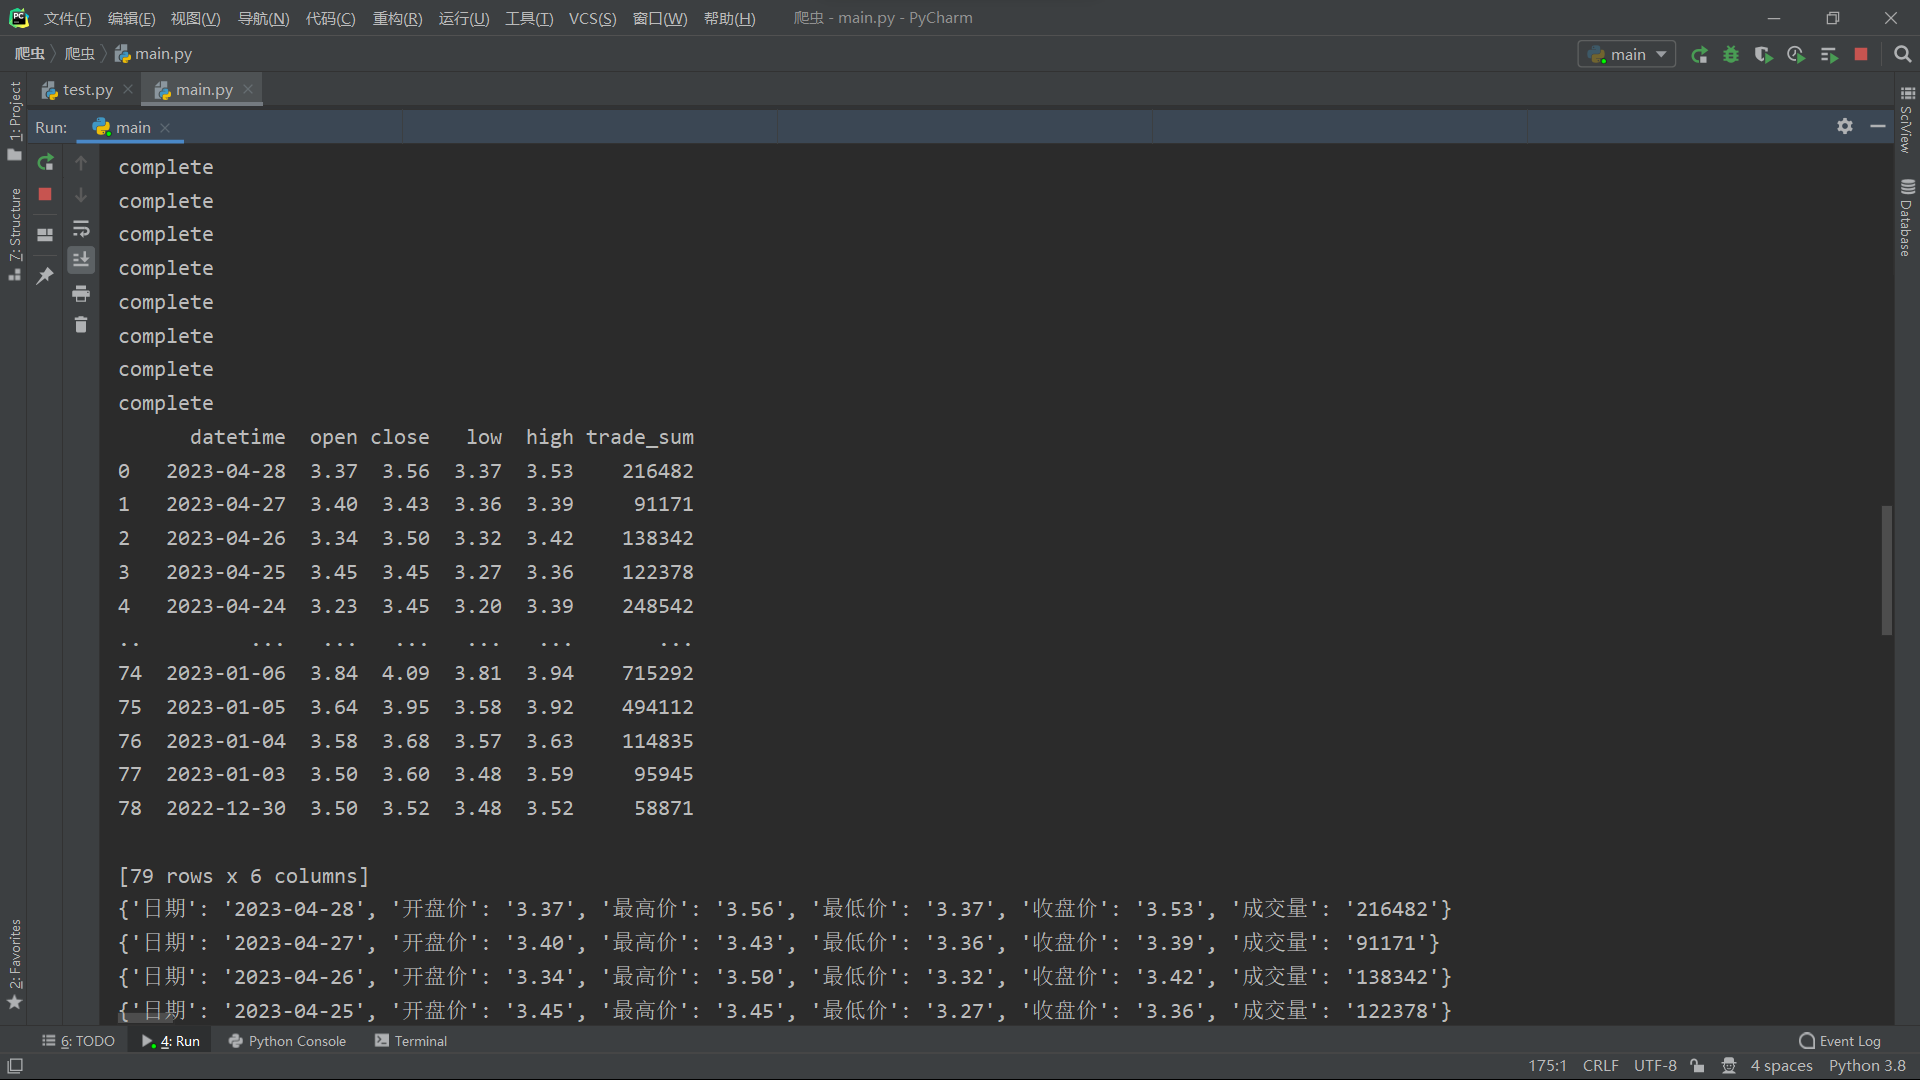
\includegraphics[width=0.9\linewidth]{img/9.png}
		\caption{控制台输出}
		\label{1}%文中引用该图片代号
	\end{minipage}
	\begin{minipage}{0.49\linewidth}
		\centering
		
\includegraphics[width=0.9\linewidth]{img/10.png}
		\caption{webdriver爬取}
		\label{2}%文中引用该图片代号
	\end{minipage}
	\qquad
	%让图片换行,
	
	\begin{minipage}{0.49\linewidth}
		\centering
		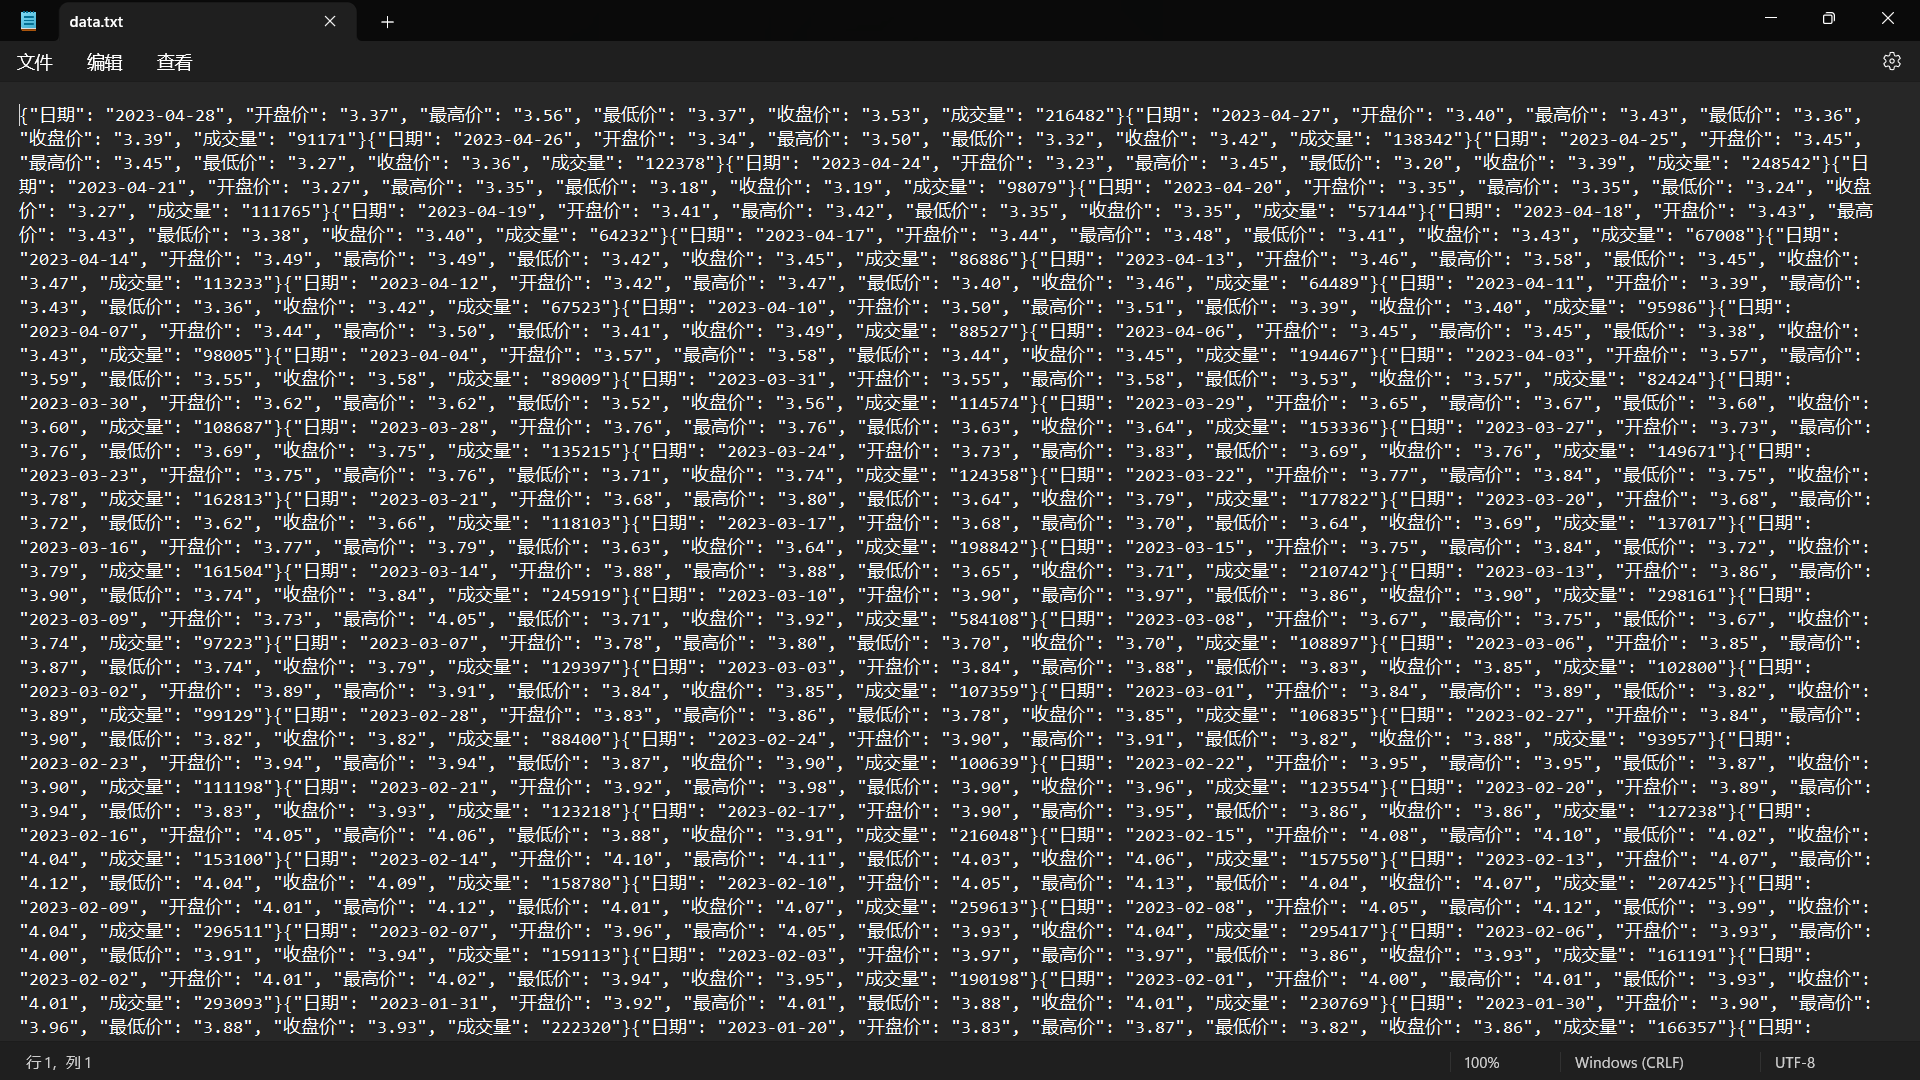
\includegraphics[width=0.9\linewidth]{img/11.png}
		\caption{txt文件生成}
		\label{3}%文中引用该图片代号
	\end{minipage}
	\begin{minipage}{0.49\linewidth}
		\centering
		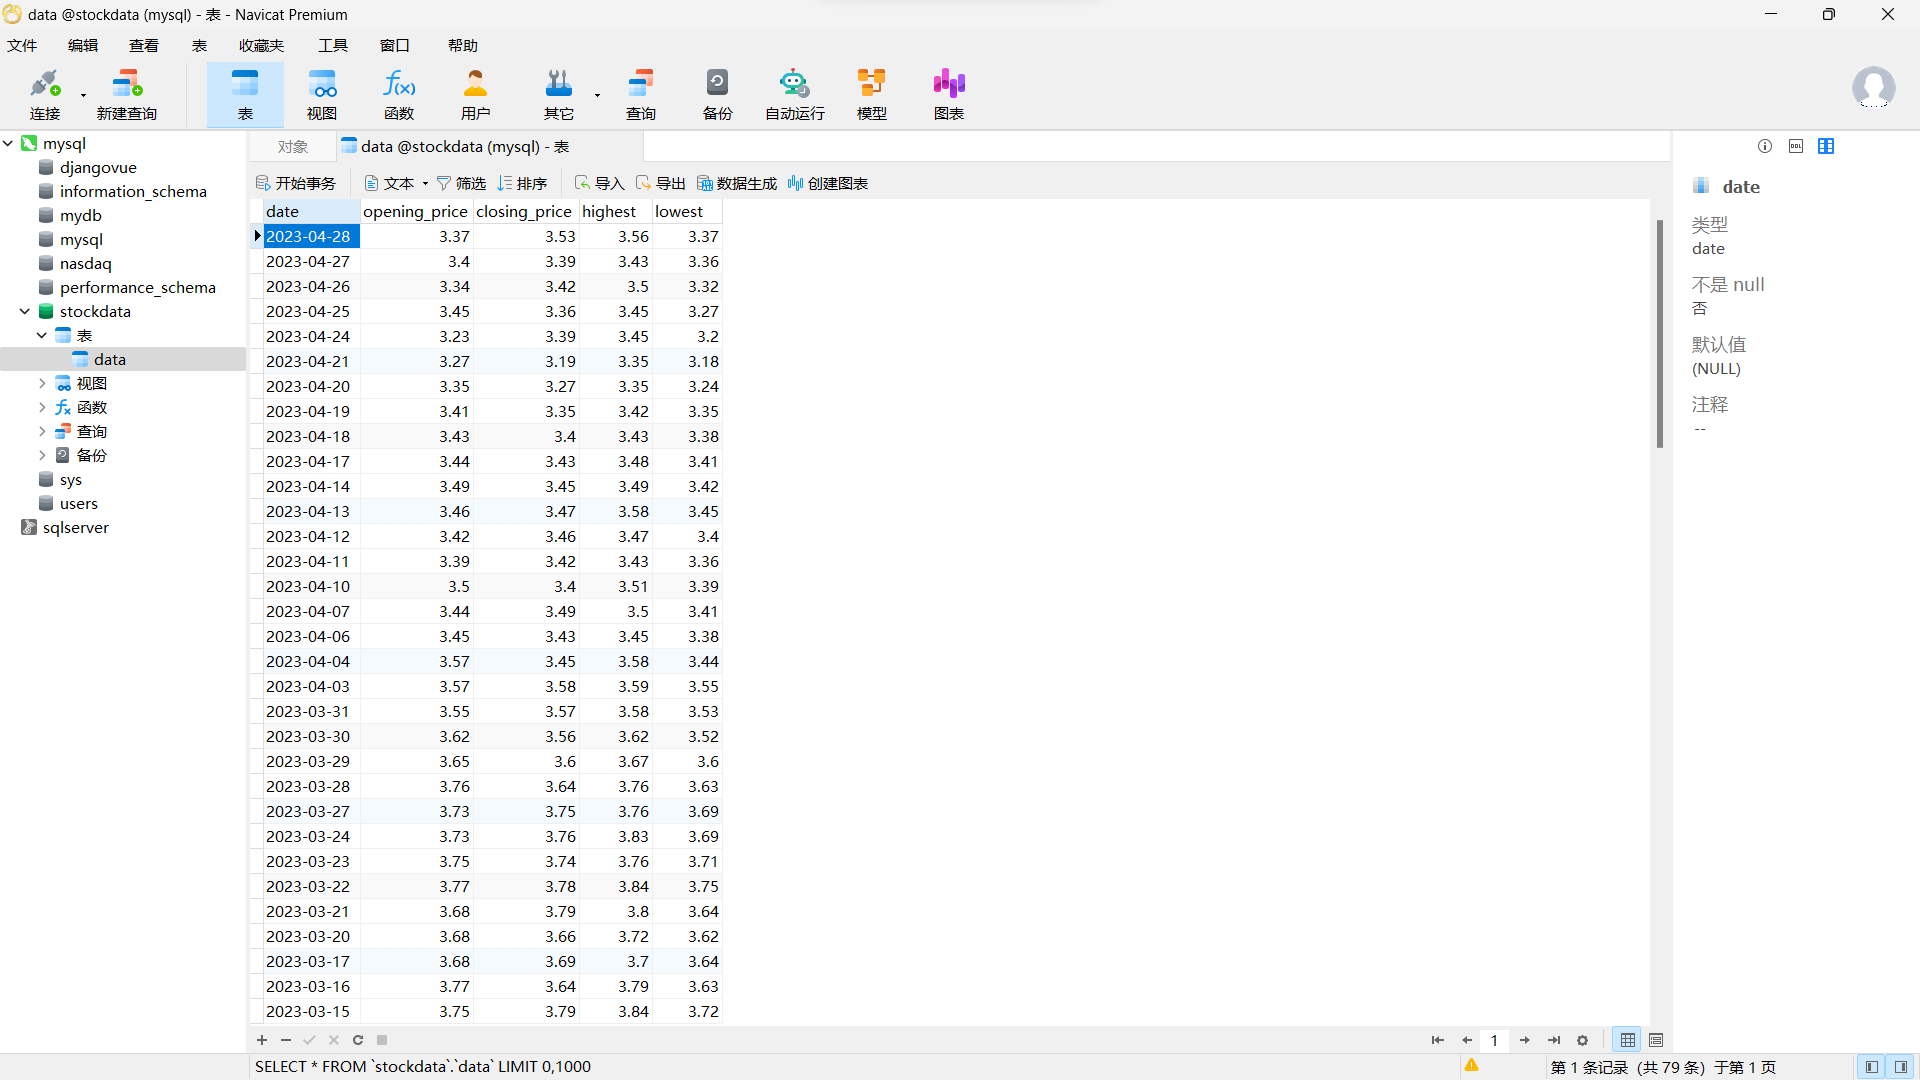
\includegraphics[width=0.9\linewidth]{img/12.png}
		\caption{数据库存储数据}
		\label{4}%文中引用该图片代号
	\end{minipage}
\end{figure}

可以看到txt文件中已经以json格式存入了数据,数据库中也存入了数据,说明程序运行正常。

\subsection{界面展示}
在界面弹出之前,程序预置爬取300117的数据,所以在界面弹出后,默认存储的是300117的数据,但是在初始界面中,是没有显示300117的数据的,需要点击“查看表格”按钮才会显示300117的数据,如图所示:

\begin{figure}[htbp]
    \centering
    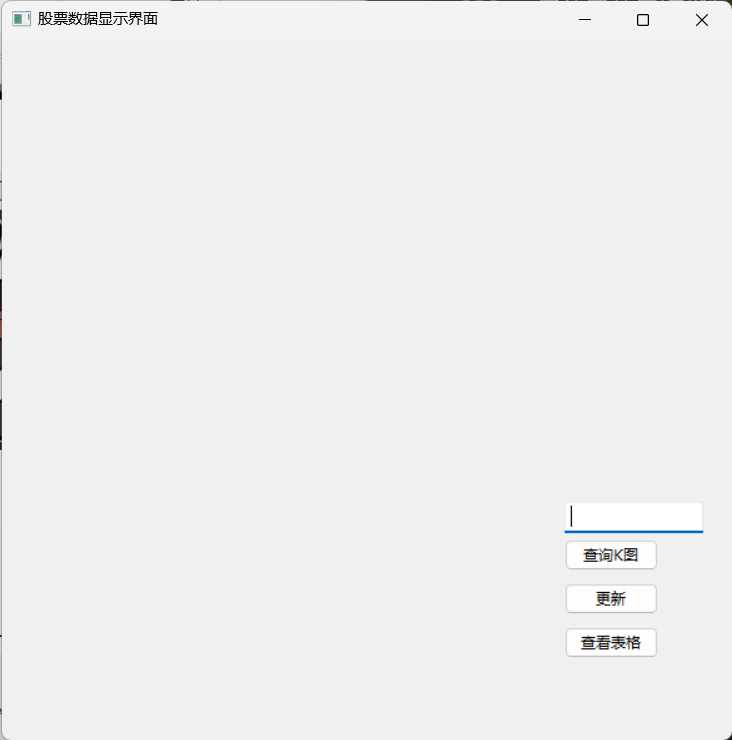
\includegraphics[width=0.3\textwidth]{img/13.png}
    \caption{初始界面显示}
\end{figure}

\subsubsection{查询表格}
首先进行表格查询,查看表格后与源数据进行比较,可以看到表格中的数据与源数据一致,说明表格查询功能正常
\begin{figure}[htbp]
    \centering
    
\includegraphics[width=0.4\textwidth]{img/8.png}
    \caption{表格展示}
\end{figure}

\subsubsection{查询K图}
点击查询K图按钮后,控制台打印输出1、查询K图,然后程序通过webbrowser.open打开浏览器,显示K线图,如图所示:
\begin{figure}[htbp]
    \centering
    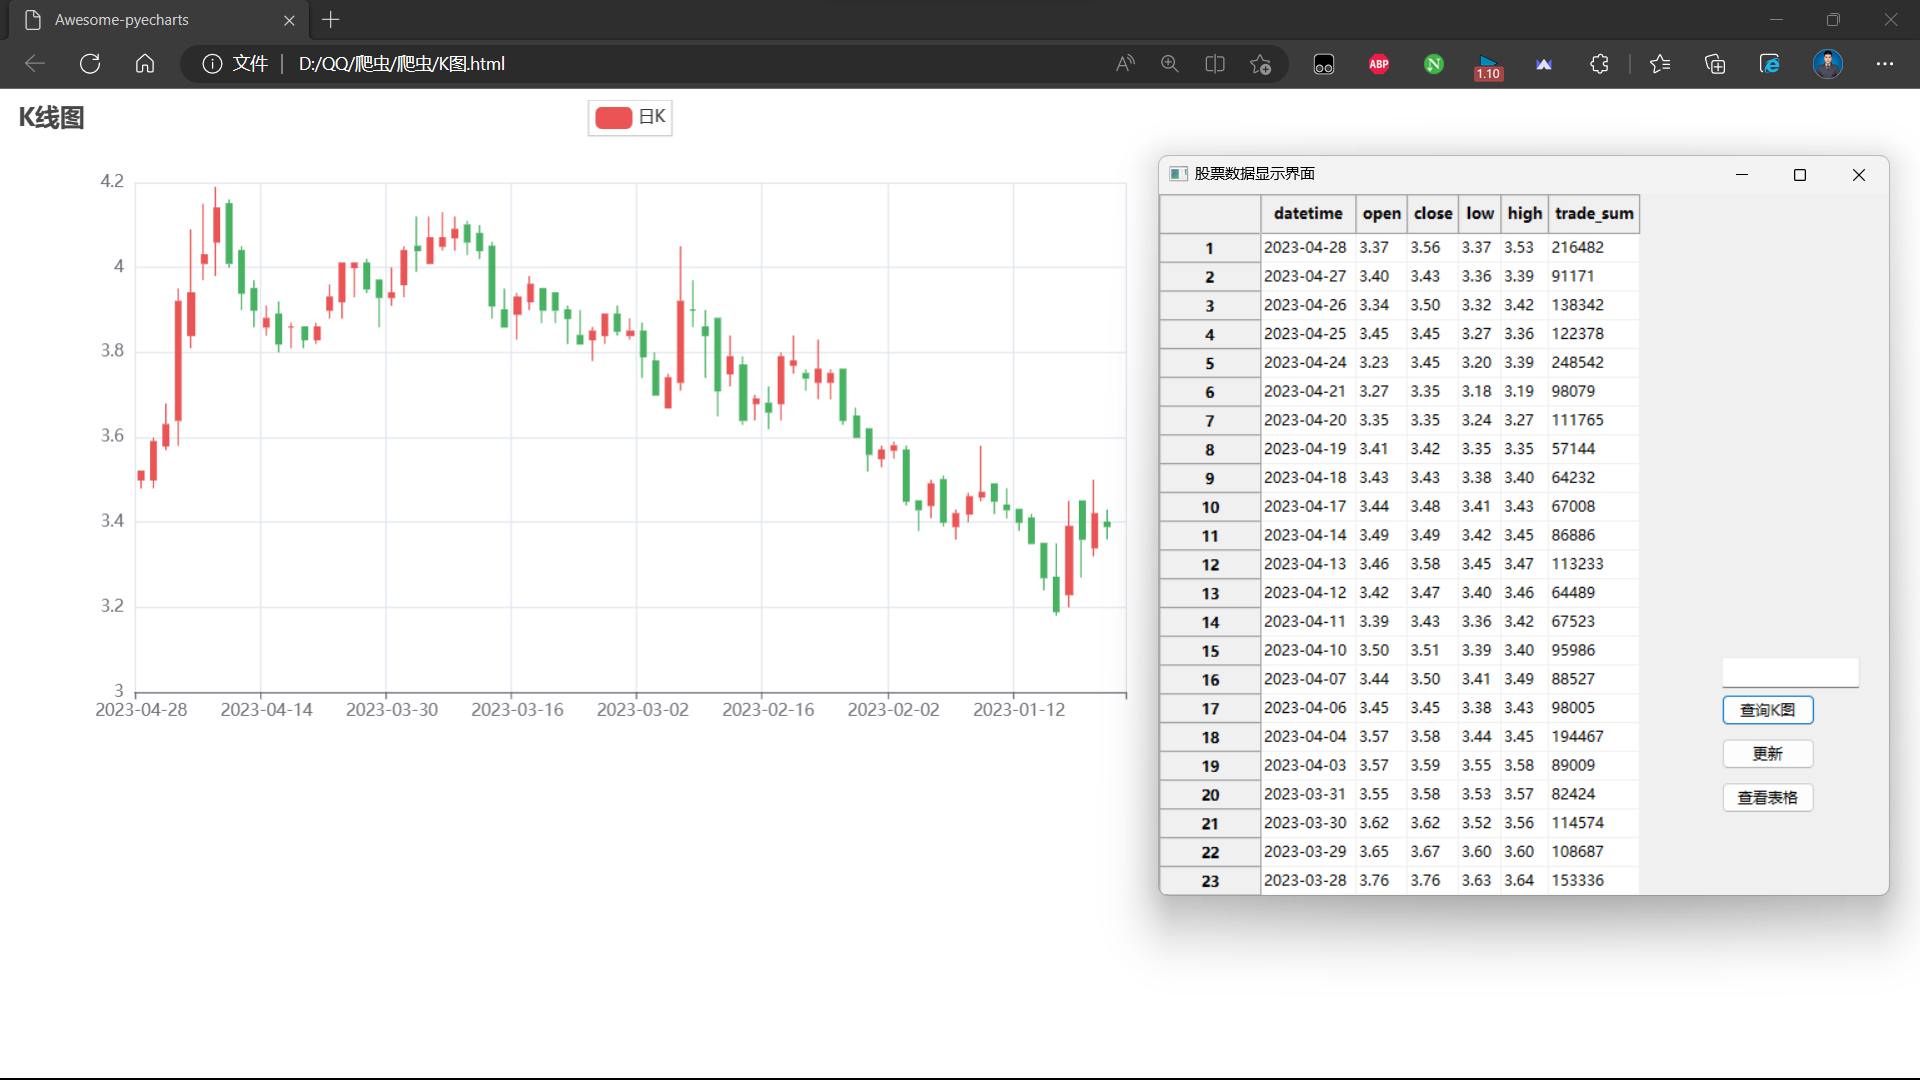
\includegraphics[width=0.6\textwidth]{img/14.png}
    \caption{K线图展示}
\end{figure}

至此,关于界面的基础展示已经展示完毕,下面将展示键入其他股票代码后的界面


\subsection{键入其他股票代码效果展示}
直接在文本框中键入其他股票代码,点击“更新”按钮,程序会对对应股票代码的历史行情数据进行重新爬取
\begin{figure}[htbp]
    \centering
    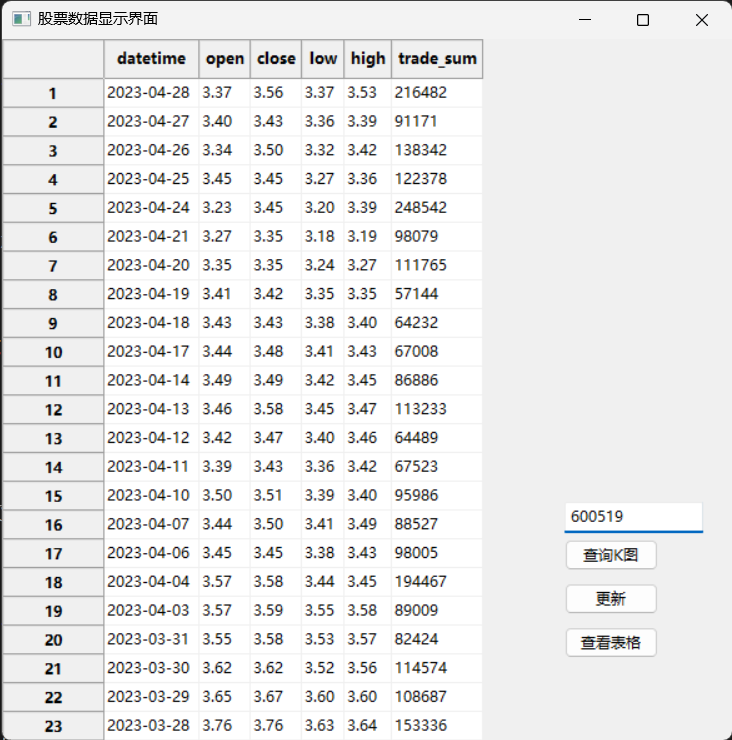
\includegraphics[width=0.6\textwidth]{img/15.png}
    \caption{键入其他股票代码}
\end{figure}

在点击更新按钮后,程序重新调用webdriver爬取对应股票代码的数据,并将数据存入数据库和txt文件中,同时在这一过程中还验证了将数据写入xlsx文件的功能,如图所示:

\begin{figure}[htbp]
	\centering
	\begin{minipage}{0.49\linewidth}
		\centering
		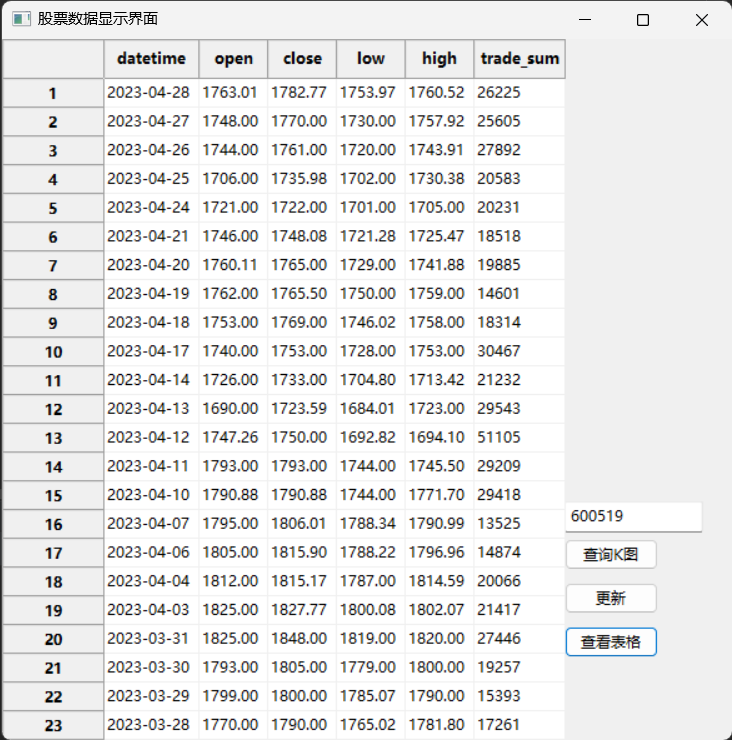
\includegraphics[width=0.4\linewidth]{img/16.png}
		\caption{更新后表格展示}
		\label{5}%文中引用该图片代号
	\end{minipage}
	\begin{minipage}{0.49\linewidth}
		\centering
		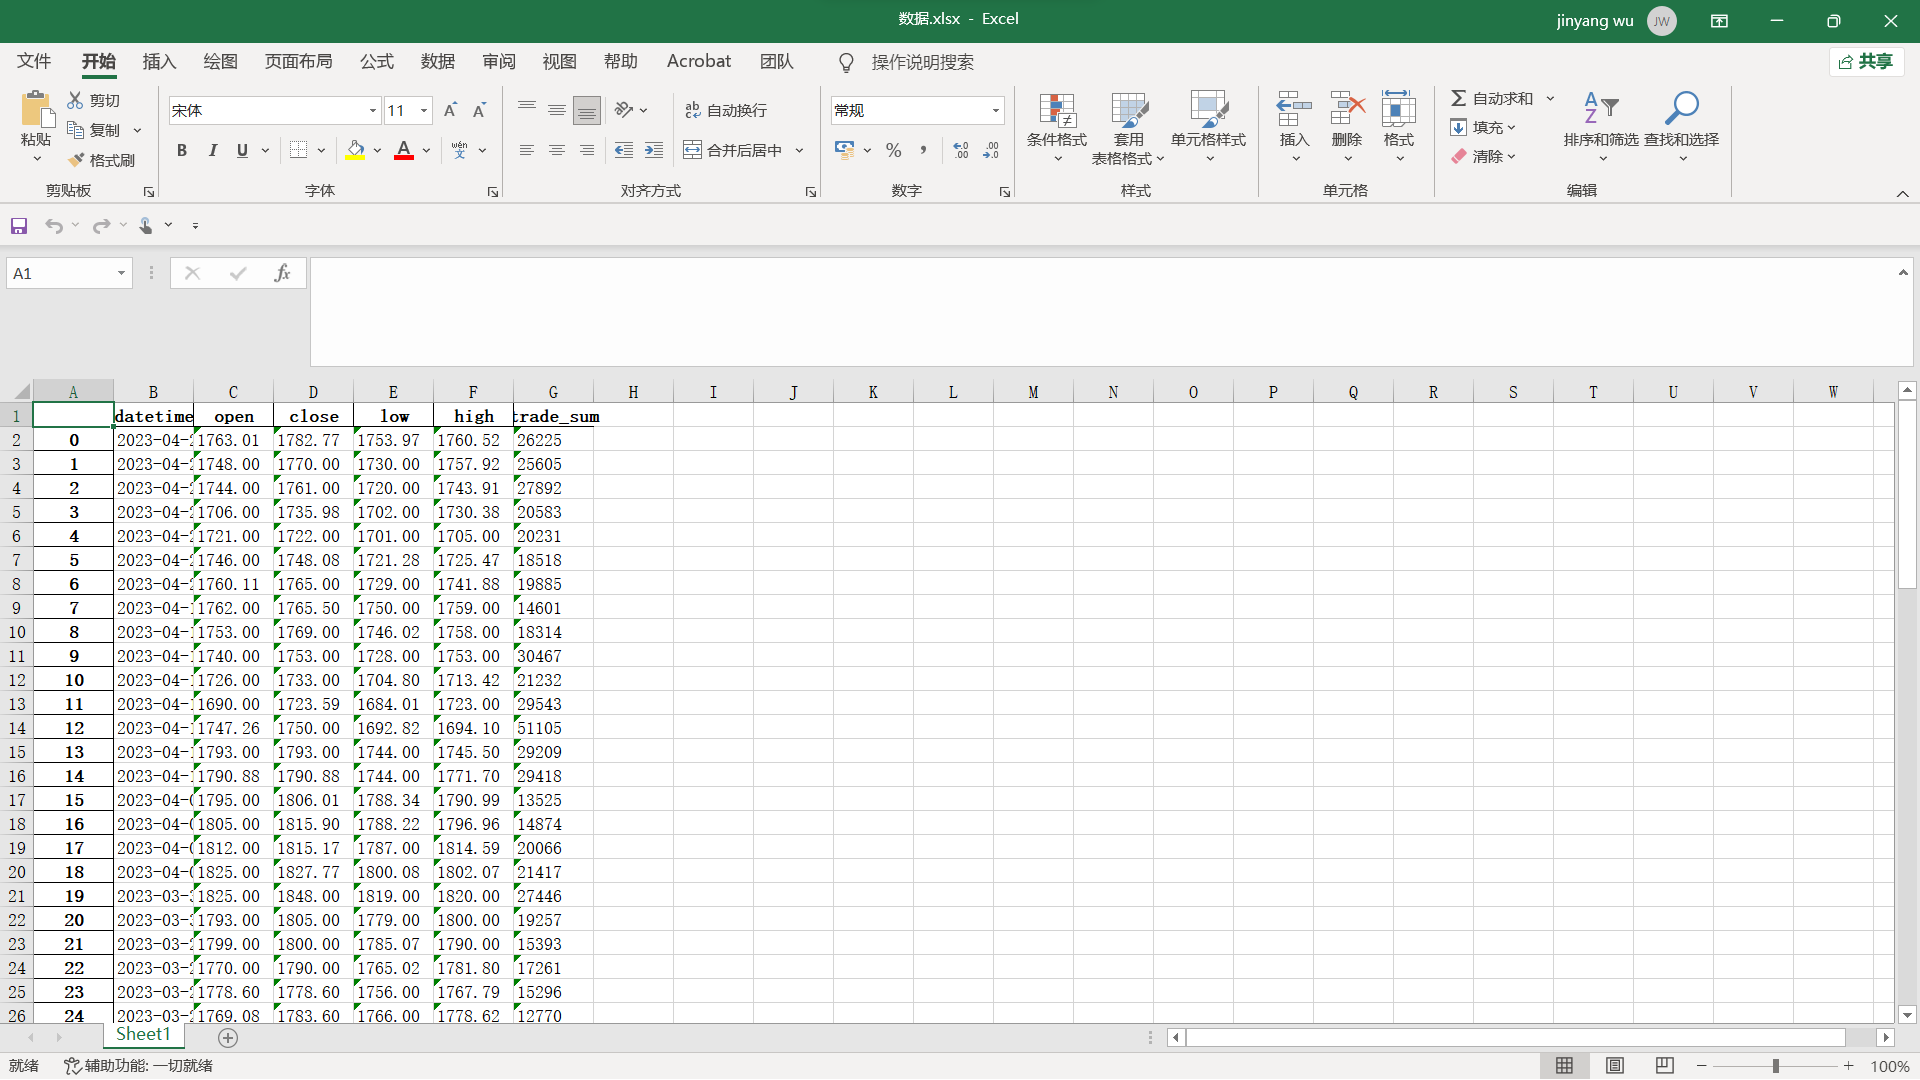
\includegraphics[width=0.9\linewidth]{img/17.png}
		\caption{xlsx文件展示}
		\label{6}%文中引用该图片代号
	\end{minipage}
	\qquad
	%让图片换行,
	
	\begin{minipage}{0.49\linewidth}
		\centering
		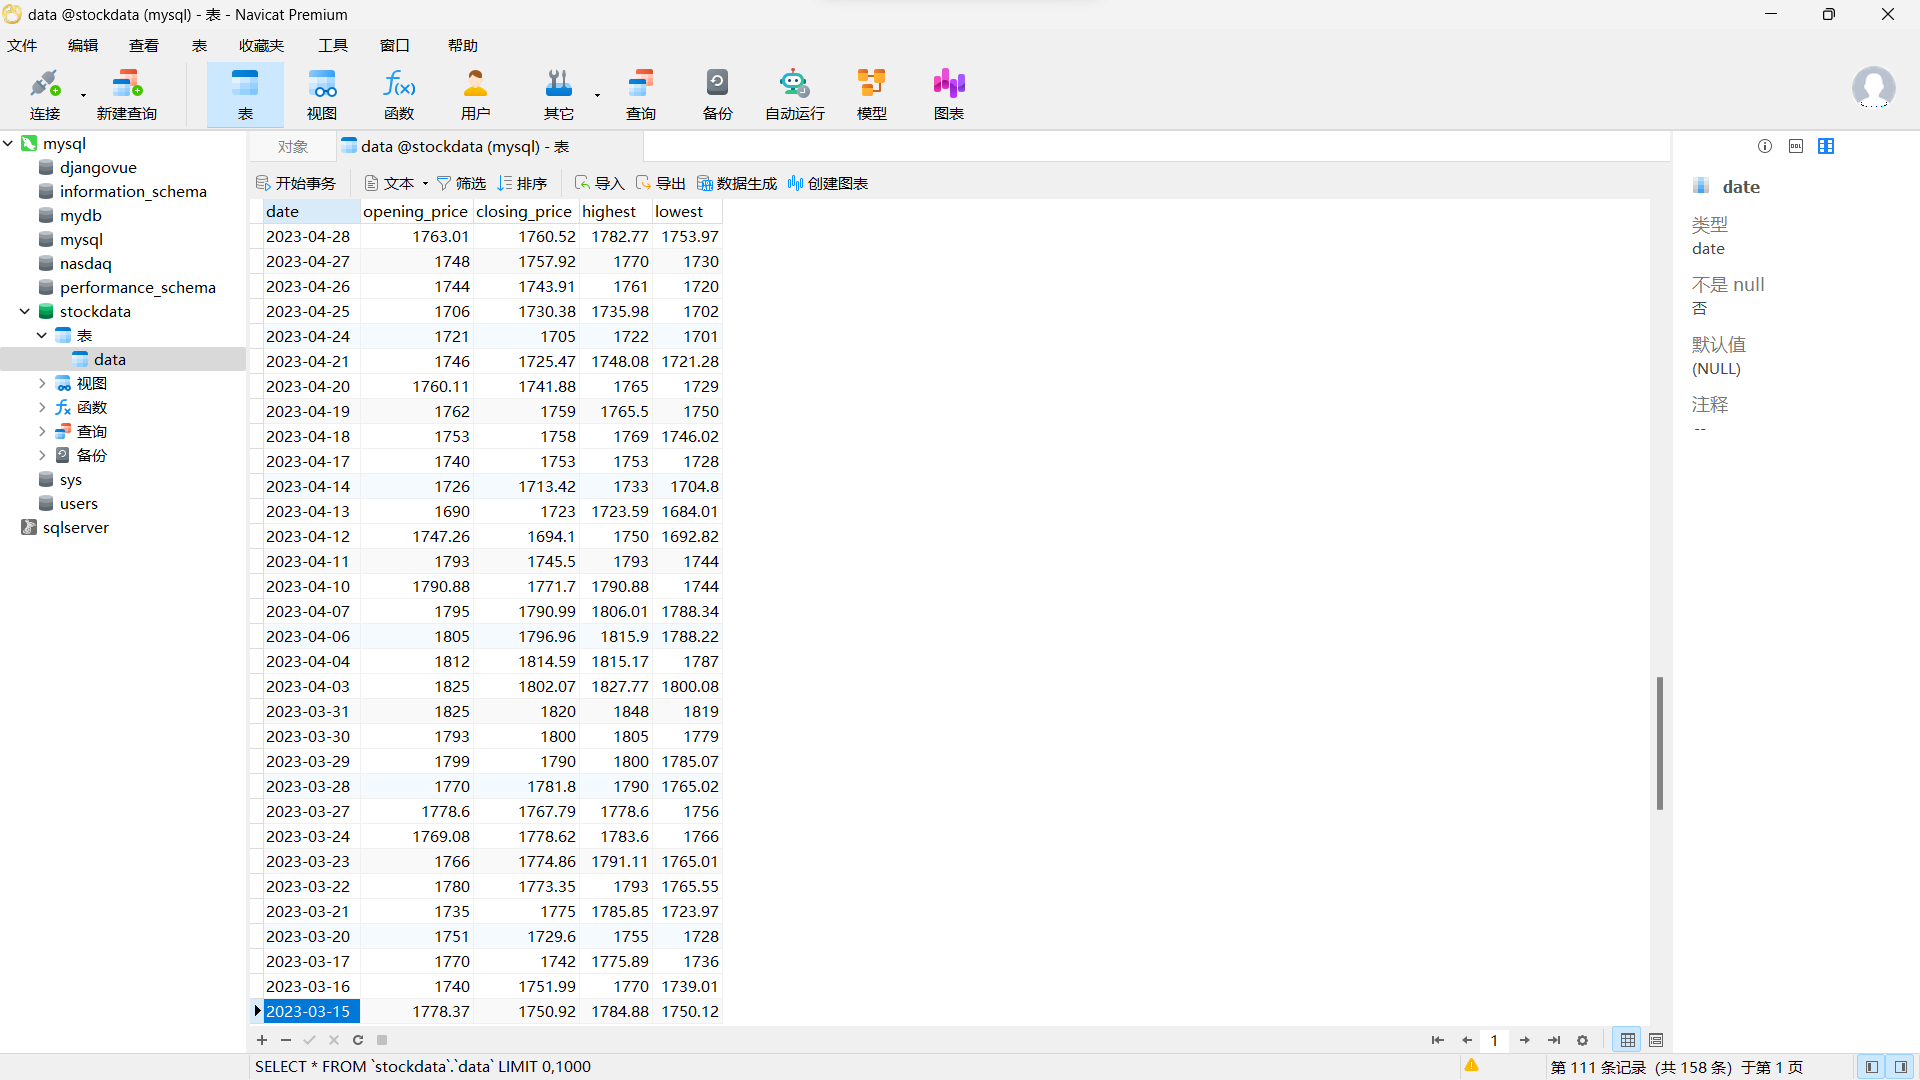
\includegraphics[width=0.9\linewidth]{img/18.png}
		\caption{数据库更新展示}
		\label{7}%文中引用该图片代号
	\end{minipage}
	\begin{minipage}{0.49\linewidth}
		\centering
		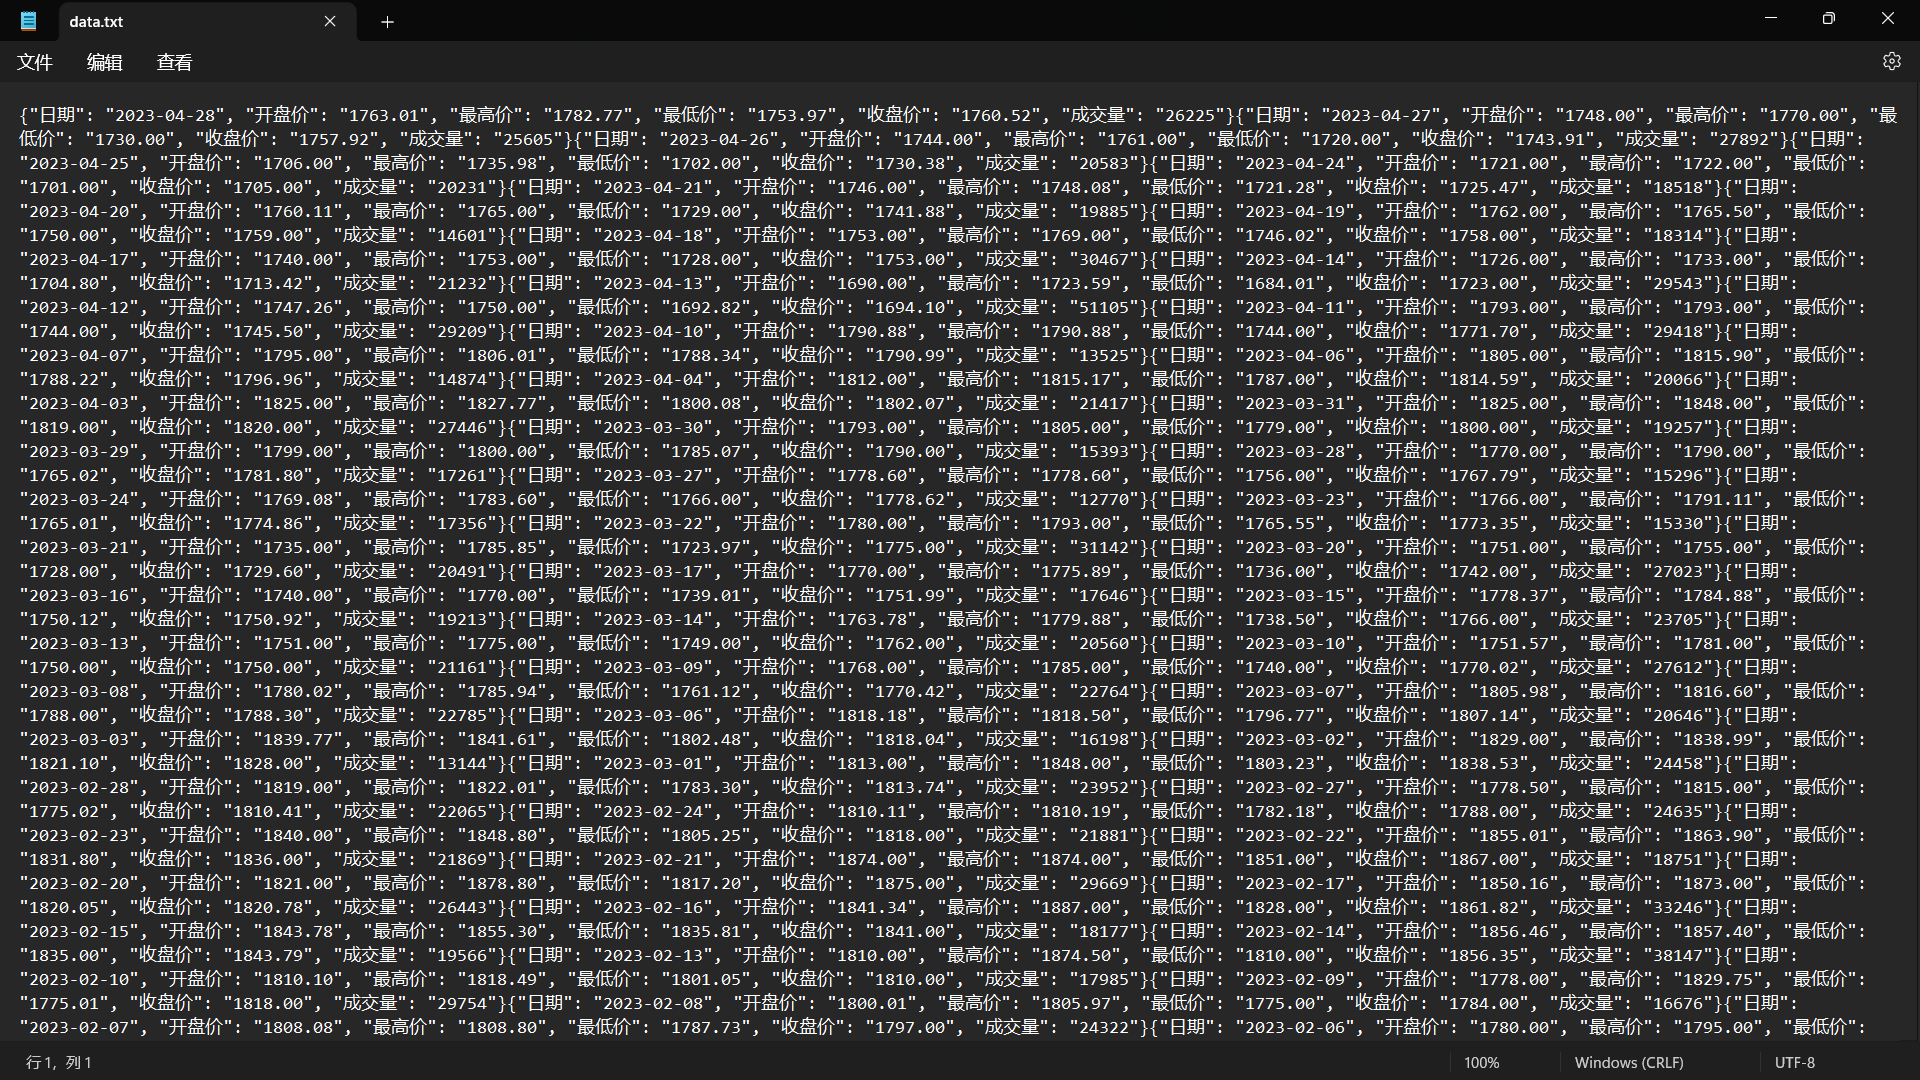
\includegraphics[width=0.9\linewidth]{img/20.png}
		\caption{txt文件展示}
		\label{8}%文中引用该图片代号
	\end{minipage}
\end{figure}

可以看到,表格、xlsx文件、数据库、txt文件中的数据都已经更新,说明更新功能正常

\subsubsection{更新查询K图效果展示}
在重新爬取数据后,数据自动更新,同时绘制K线图的函数也被自动调用,点击查询K图按钮可以看到更新后的K线图,如图所示:

\begin{figure}[htbp]
    \centering
    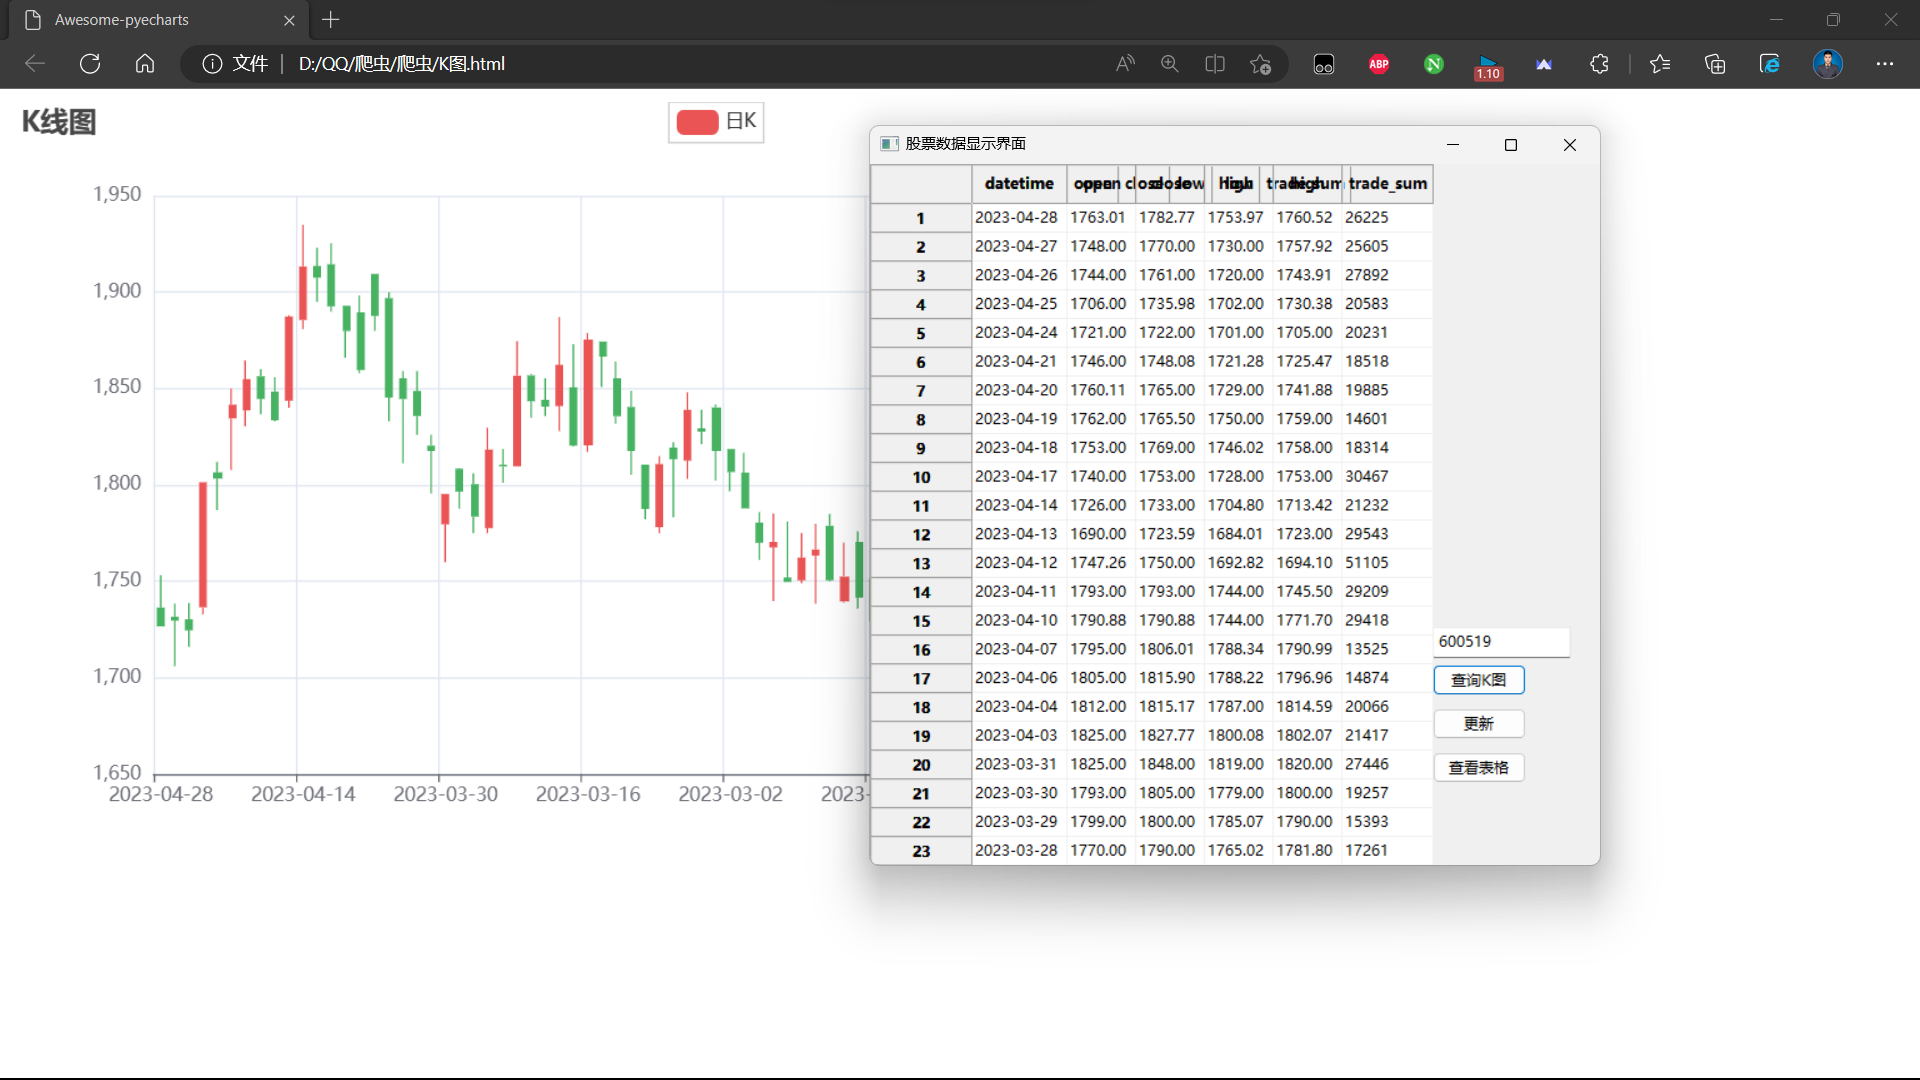
\includegraphics[width=0.5\textwidth]{img/19.png}
    \caption{更新K线图展示}
\end{figure}

至此,本实验的所有功能基本展示完毕

\section{总结}
本次实验涉及到了python爬虫、数据库、图像绘制技术以及python制作GUI界面等相关知识,综合性比较强,学习到的新知识也非常多
\subsection{关于爬虫}
在最开始爬取股票的历史行情数据的时候,并不知晓其历史行情数据采用动态方式,在最开始的时候获取数据使用了request库获取了静态的html文件,
\begin{lstlisting}
# def getHtml(stack_code):
#     data = requests.get("https://q.stock.sohu.com/cn/" +
#     stack_code + "/lshq.shtml",
#     headers={"user-agent": "Mozilla/5.0 (Windows NT 10.0; Win64; x64) AppleWebKit/537.36 (KHTML, like Gecko) Chrome/112.0.0.0 Safari/537.36 Edg/112.0.1722.58"})
#     # 获得一个请求得到的静态网页
#     return data.text


# 将HTML文本转化成字典列表
# def getData(data):
#     month_data = []
#     soup = BeautifulSoup(data, "lxml")  # data由getHtml()取得
#     # 爬取网页的工具
#     list = soup.find("div", class_="part").find("table", class_="tableQ")
#     # 看html,已经把不需要的都删了,数据在innerbox的table_bg001 border_box limit_sale下面
#     dataList = list.find_all("tr")[1:]
#     # 因为第一个tr后面是一堆th标签,不需要
#     f = open("data.txt", "w", encoding="utf-8")
\end{lstlisting}
\begin{lstlisting}[title=request库调取,frame=shadowbox]
#     for item in dataList:
#         kv = {}
#         if isinstance(item, bs4.element.Tag):
#             tdList = item.find_all("td")
#             # print(tdList)
#             kv["日期"] = tdList[0].text  # 去掉td和/td,取中间的内容
#             kv["开盘价"] = tdList[1].text
#             kv["最高价"] = tdList[6].text
#             kv["最低价"] = tdList[5].text
#             kv["收盘价"] = tdList[2].text
#             kv["成交量"] = tdList[7].text
#         month_data.append(kv)
#         to_write = json.dumps(kv,ensure_ascii=False)
#         f.write(to_write)
#         # print(kv)
#     f.close()
#     # print(month_data)  # 字典列表
#     return month_data
\end{lstlisting}
反复试验后无法获得相应数据,通过分析html的源代码(股票代码300117的界面html源码见附录),发现tbody标签中元素为空,分析确定静态文件中没有数据,因此使用selenium库中的webdriver模块获取动态数据,通过分析动态数据,最终成功获取数据,但是在获取数据的过程中,由于数据量较大,程序运行时间较长,所以在获取数据的过程中,需要设置等待时间,否则会出现获取不到数据的情况,最终通过设置等待时间解决了这一问题,同时在获取数据的过程中,由于数据量较大,所以需要设置浏览器的窗口大小,否则会出现数据不全的情况,最终通过设置浏览器窗口大小解决了这一问题,最终成功获取了数据


\subsection{关于可视化界面}
本实验使用了wxpython库来实现项目的GUI界面,在实现过程中,只搭建了了一个简单的框架,但是麻雀虽小五脏俱全,满足了基本功能

\subsection{关于绘图}
在绘图的时候,没有选择matplotlib库,选用了pyecharts库,其中的Kline类能够直接实现K线图的绘制。

但是在绘制的时候,发现pyecharts库的Kline类只能绘制一只股票的K线图,所以在绘制新股票的时候,需要重新读取元素绘制,最终实现了另一个K线图的绘制,同时覆盖了上一个元素的K线图,实现了K线图的更新。

\subsection{关于数据库}
本实验中,调用pymysql库实现了数据库的连接,通过数据库的连接,实现了数据的存储,同时在更新数据的时候,也实现了数据的更新,最终实现了数据的存储和更新。在实验过程中,由于数据库的连接需要设置host、user、password、database等参数,所以在实验过程中,需要设置这些参数,否则会出现连接不上数据库的情况,最终通过设置这些参数解决了这一问题,成功连接了数据库。此外还学习了cursor游标的使用,通过游标实现了数据的插入和更新。

\section{附录}

\subsection{股票代码300117的界面html源码}
\begin{lstlisting}[title=股票代码300117的界面html源码,frame=shadowbox]
    <!DOCTYPE html PUBLIC "-//W3C//DTD XHTML 1.0 Transitional//EN" "http://www.w3.org/TR/xhtml1/DTD/xhtml1-transitional.dtd">
    <html xmlns="http://www.w3.org/1999/xhtml">
    <head>
    <meta http-equiv="Content-Type" content="text/html; charset=gb2312" />
    <title>贵州茅台(600519) - 历史行情 - 股票行情中心 - 搜狐证券</title>
    <meta name="Keywords" content="贵州茅台,600519,历史行情">
    <meta name="Description" content="贵州茅台(600519)的历史行情,提供贵州茅台(600519)的历史行情等信息">
    <link type="text/css" rel="stylesheet" href="//s1.biz.itc.cn/cn/css/BIZ_comm-1.4.2.css?000" media="screen" />
    <link type="text/css" rel="stylesheet" href="//k.sohu.com/static/finance/pc/qstock/v0.0.12/css/BIZ_sec-1.4.1.css" media="screen" />
    
    <script type="text/javascript">
    /* 文件生成时写入区域 START */
    biz_Code = "cn_600519";
    //正常状态:0,选中状态:1,无效置灰状态:-1
                //上市股票
                    biz_leftMenuConfig = [[0],[0, 0, 0, 0, 0, 0],[0],[0, 0, 0, 0, 0, 0],[0, 0, 0, 0],[0, 0, 0, 0, 0, 0, 0]];
        
    biz_leftMenuConfig[1][3]=1;
                                            biz_middMenuConfig = [0,0,0,1,-1,0];
                            /* 文件生成时写入区域 END */
    </script>
    <!-- 头部js START -->
    <script type="text/javascript" src="//s1.biz.itc.cn/cn/script/lib/jquery-1.7.2.js"></script> 
    <script type="text/javascript" src="//s4.biz.itc.cn/cn/script/mystock/JCalendar-1.js"></script>
    <script type="text/javascript">
    var BIZ_menu_config = { nav: 1 };
    commet_obj = {};
    var loadEvents = function(){
        //行情
        var ml1 = new jaw.commet();
        commet_obj = ml1;
        ml1.append("hq2", 25, PEAK.getHqURL(2));
        ml1.handler();
        
        var url = PEAK.BIZ.HOST + "/hisHq?code="+biz_Code+"&stat=1&order=D&period=d&callback=historySearchHandler&rt=jsonp";
        jaw.evalScript({url: url});
    
        var jCalendar = new JCalendar();
        jCalendar.bind("BIZ_lshq_sd", "bottom");
        jCalendar.bind("BIZ_lshq_ed", "bottom");
    }
    </script>
    <script type="text/javascript" src="//k.sohu.com/static/finance/pc/qstock/v0.0.10/js/main/autocomplete.min.js"></script>
    <script type="text/javascript" src="//k.sohu.com/static/finance/pc/qstock/v0.0.10/js/main/main-1.4.7.min.js"></script>
    <script type="text/javascript" src="//k.sohu.com/static/finance/pc/qstock/v0.0.10/js/main/hq_sec-1.4.min.js"></script>
    <style style="text/css">
    #calendar_container { width:160px;border:1px solid #06C}
    #calendar {border-collapse:collapse;background-color:#FFF;width:160px;height:120px;margin:0px auto}
    #calendar td {font-size:12px;text-align:center;vertical-align:middle;font-family:"宋体"}
    #calendar thead {background-color:#999;color:#FFF}
    #calendar thead tr td{font:bold;height:20px;}
    #calendar caption {background-color:#06C;height:20px;padding:3px 0 0 2px;*padding:5px 0 0 3px}
    #calendar a{color:#F90;margin:0 5px;text-decoration:none}
    #calendar #prev_month,#calendar #next_month {font-size:18px;margin:0}
    #calendar #c_today {background-color:#036;color:#FFF}
    #calendar span.arrowL {background:#EEF5FF;width:14px;height:14px;border:1px #07C solid;position:absolute;top:3px;left:12px;cursor:pointer}
    #calendar span.arrowL em {*font-size:1px;width:0;height:0;border:5px #EEF5FF solid;border-right:5px #07C solid;position:absolute;top:2px;*top:0;left:0;*border:5px #EEF5FF solid;*border-right:4px #07C solid}
    #calendar span.arrowR {background:#EEF5FF;width:14px;height:14px;border:1px #07C solid;position:absolute;top:3px;left:132px;cursor:pointer}
    #calendar span.arrowR em {*font-size:1px;width:0;height:0;border:5px #EEF5FF solid;border-left:5px #07C solid;position:absolute;top:2px;*top:1px;left:4px;*left:3px;*border:4px #EEF5FF solid;*border-left:5px #07C solid}
    #calendar .over {background-color:#CCC}
    #calendar .keydate {color:#06F}
    </style>
    
    <!-- 头部js END -->
    </head>
    
    <body>
    
    <!-- 页头 START -->
    <!-- 搜狐通用页眉A START -->
    <div id="criterionNav" class="Area_w">
        <a target="_blank" href="//www.sohu.com/" id="sohu_logo"><img height="22" border="0" src="//s1.biz.itc.cn/cn/pic/sohu_logo2.gif" alt="搜狐网站"/></a>
        <a target="_blank" href="//stock.sohu.com/" id="sohu_sec_logo"><img height="22" border="0" src="//s2.biz.itc.cn/cn/pic//stock_logo2.gif" alt="搜狐证券"/></a>
    
        <div id="criterionNav_right" class="Area">
        <ul class="right">
            <li><a target="_top" href="//www.sohu.com/">搜狐首页</a></li>
            <li>-</li>
            <li class="red"><a target="_top" href="//news.sohu.com/">新闻</a></li>
            <li>-</li>
            <li><a target="_top" href="//sports.sohu.com/">体育</a></li>
            <li>-</li>
            <li><a target="_top" href="//s.sohu.com/">S</a></li>
            <li>-</li>
            <li><a target="_top" href="//yule.sohu.com/">娱乐</a></li>
            <li>-</li>
            <li><a target="_top" href="//v.sohu.com/">V</a></li>
            <li>-</li>
            <li class="red"><a target="_top" href="//business.sohu.com/">财经</a></li>
            <li>-</li>
            <li><a target="_top" href="//it.sohu.com/">IT</a></li>
            <li>-</li>
            <li><a target="_top" href="//auto.sohu.com/">汽车</a></li>
            <li>-</li>
            <li><a target="_top" href="//house.sohu.com/">房产</a></li>
            <li>-</li>
            <li><a target="_top" href="//home.sohu.com/">家居</a></li>
            <li>-</li>
            <li><a target="_top" href="//women.sohu.com/">女人</a></li>
            <li>-</li>
            <li><a target="_top" href="//tv.sohu.com/">视频</a></li>
            <li>-</li>
            <li><a target="_top" href="//v.blog.sohu.com/">播客</a></li>
            <li>-</li>
            <li><a target="_top" href="//www.chinaren.com/">ChinaRen</a></li>
            <li>-</li>
            <li><a target="_top" href="//login.mail.sohu.com/">邮件</a></li>
            <li>-</li>
            <li><a target="_top" href="//blog.sohu.com/">博客</a></li>
            <li>-</li>
            <li><a target="_top" href="//club.sohu.com/">BBS</a></li>
            <li>-</li>
            <li><a target="_top" href="//comment2.news.sohu.com/">我说两句</a></li>
            <li>-</li>
            <li class="end"><a target="_top" href="//www.sogou.com/">搜狗</a></li>
        </ul>
        </div>
    
    </div>
    <!-- 搜狐通用页眉A END -->
    
    <!-- 行情中心页眉 START -->
    <div class="BIZ_header">
        <img id="BIZ_logo" src="//s3.biz.itc.cn/cn/pic/logo_BIZ_new_1.4.gif" title="搜狐财经行情Logo" alt="搜狐财经行情Logo" usemap="#BIZ_logo" />
        <map name="BIZ_logo">
            <area shape="rect" coords="0,0,110,46" href="//stock.sohu.com/" target="_blank"></area>
            <area shape="rect" coords="110,0,200,46" href="//q.stock.sohu.com/" target="_blank"></area>
        </map>
        <div id="BIZ_ver">
         <!--	<a style="padding-right:30px;color:#f00" href="//stock.sohu.com/20130428/n374361532.shtml" target="_blank">*声明:由于系统调整,暂停美股港股行情服务</a> -->
            <a target="_blank" href="//q.stock.sohu.com/feedback.html">意见反馈</a>
            <a target="_blank" href="//stock.sohu.com/upload/stock_mobile.html " style="color:#18479B;">手机随时随地看行情</a>
        </div>
    
        <!-- 顶部功能栏 START -->
        <ul id="BIZ_fnbarA" class="BIZ_fnbarA">
            <li class="e1" c=0><a href="javascript:addBookmark();">加入收藏夹</a></li>
            <li class="e2" c=1><a href="javascript:setHomepage();">设为首页</a></li>
        </ul>
        <!-- 顶部功能栏 END -->
    
        <!-- 行情中心主导航 START -->
        <style type="text/css">
        div.BIZ_header div.BIZ_nav ul li{margin-right:0}
        </style>
        <div id="BIZ_nav" class="BIZ_nav">
            <ul style="width:900px;margin-left:135px">
                <li>首 页<a href="/index.shtml">首 页</a></li>
                <li>个 股<a href="/cn/000002/index.shtml">个 股</a></li>
                <li>指 数<a href="/cn/zs.shtml">指 数</a></li>
                <li>排 行<a href="/cn/ph.shtml">排 行</a></li>
                <li>板 块<a href="/cn/bk.shtml">板 块</a></li>
                <li>自选股<a style="background:url(//stock.sohu.com/upload/mystock2012/html/skin/images/new2.gif) no-repeat" href="/cn/mystock.shtml">自选股</a></li>
            <!--	<li>千股千评<a href="//t.stock.sohu.com">千股千评</a></li>-->
            <!--	<li>炒股大赛<a href="//q.stock.sohu.com/cgds/" target="_blank" style="color:#f60">炒股大赛</a></li>-->
            </ul>
            <div class="BIZ_update_info" style="display:none"></div>
            <div class="BIZ_nav_border"></div>
        </div>
    </div>
    <!-- 行情中心页眉 END -->
    
    <!-- 页头 END -->
    
    <!-- 行情中心主栏 START -->
    <style type="text/css">
        div#FEP_searchbar{left:15px}
        div.BIZ_bar_wrapper div.BIZ_bar div.BIZ_login ul.off li.fn{width:50px;}
        div.BIZ_bar_wrapper div.BIZ_bar div.BIZ_login ul.on li.caption{margin-right:10px}
        div.BIZ_bar_wrapper div.BIZ_bar div.BIZ_login{left:auto;right:10px;background:url(//i1.itc.cn/20120920/2bb1_e4c60ac2_b96d_b596_71aa_d67fed8c8861_1.png) no-repeat; _background:transparent;_filter:progid:DXImageTransform.Microsoft.AlphaImageLoader(enabled='true',sizingMethod='crop',src='//i1.itc.cn/20120920/2bb1_e4c60ac2_b96d_b596_71aa_d67fed8c8861_1.png')}
    </style>
    <div class="BIZ_bar_wrapper">
        <div id="BIZ_bar" class="BIZ_bar">
            <!--
            <span class="BIZ_user"></span>
            行情中心登陆元素 START -->
            <div id="BIZ_login" class="BIZ_login"></div>
            <!-- 行情中心登陆元素 END -->
            
            <!-- 搜索&Suggest START -->
            <div id="FEP_searchbar" class="searchbar suggestRoot clearfix">
                <form action="javascript:void(0)" id="searchForm">
                    <ul id="FEP_searchList" class="searchList clearfix">
                        <li class="e1"><input id="searchInput" type="text" autoComplete="off" disableautocomplete /></li>
                        <li class="e2"><input id="FEP_searchBtn" type="submit" class="suggest_btn" value=""/></li>
                    </ul>
                </form>
                <div id="suggestDiv" class="suggestLists" style="display: none; "></div>
            </div>
            <!-- 搜索&Suggest END -->
        </div>
        <div class="BIZ_bar_border"></div>
    </div>
    <!--<div class="flash" style="width:980px;margin:0 auto 10px">
        <a href="//q.stock.sohu.com/cgds/index.do" target="_blank"><img src="//stock.sohu.com/upload/chaogu_pc/images/gf980x100.gif"></a>
    </div>-->
    
    <!-- 行情中心主栏 END -->
    
    <div class="str2Column clearfix">
        <div class="str2ColumnL">
            <!-- 行情中心主菜单 START -->
            <div class="BIZ_menu_shadow">
                <div id="BIZ_stock_list" class="BIZ_stock_list">
        <div class="BIZ_tabA">
            <ul class="clearfix" id="FTag">
                <li id="ft0" class="current" c="BIZ_MyLBS"><span>最近浏览股</span></li>
                <li id="ft1" c="BIZ_Mystock"><span><a href="//q.stock.sohu.com/cn/mystock.shtml">我的自选股</a></span></li>
            </ul>
        </div>
        <table id="BIZ_MyLBS">
            <tr><td width="50px"><span>&nbsp;</span></td><td></td></tr>
            <tr><td><span>&nbsp;</span></td><td></td></tr>
            <tr><td><span>&nbsp;</span></td><td></td></tr>
            <tr><td><span>&nbsp;</span></td><td></td></tr>
            <tr class="last"><td><span>&nbsp;</span></td><td></td></tr>
        </table>
        <table id="BIZ_Mystock" style="display:none">
            <tr><td width="50px"><span>&nbsp;</span></td><td></td></tr>
            <tr><td><span>&nbsp;</span></td><td></td></tr>
            <tr><td><span>&nbsp;</span></td><td></td></tr>
            <tr><td><span>&nbsp;</span></td><td></td></tr>
            <tr class="last"><td><span>&nbsp;</span></td><td></td></tr>
        </table>
    </div>
    
    <div class="BIZ_menu_border">
        <div id="BIZ_menu" class="BIZ_menu">
    <script>biz_Name = "贵州茅台";
    var status = "0";</script>
    <div class="part first">
        <ul>
            <li><a href="//q.stock.sohu.com/cn/600519/index.shtml"><b>贵州茅台</b></a></li>
        </ul>
    </div>
        <div class="part">
            <h3>行情图表</h3>
            <ul>
                <li class="tuijian_li" style="display:none"><a href="//q.stock.sohu.com/qp/index.html?cn_600519">实时行情</a><span class="tuijian">推荐</span></li>
                <li><a href="//q.stock.sohu.com/cn/600519/cjmx.shtml">成交明细</a></li>
                <li><a href="//q.stock.sohu.com/cn/600519/fjb.shtml">分价表</a></li>
                <li><a href="//q.stock.sohu.com/cn/600519/lshq.shtml">历史行情</a></li>
                <li><a href="//q.stock.sohu.com/cn/600519/lhb.shtml">龙虎榜数据</a></li>
                                <li><a href="//q.stock.sohu.com/cn/600519/dzjy.shtml">大宗交易</a></li>
                        </ul>
        </div>
        <div class="part">
            <h3>新闻资讯</h3>
            <ul>
                <!-- <li><a href="//q.stock.sohu.com/cn/600519/news_gs.shtml">公司新闻</a></li> -->
                <li><a href="//q.stock.sohu.com/cn/600519/gsgg.shtml">公司公告</a></li>
                <!-- <li><a href="//q.stock.sohu.com/cn/600519/news_gg.shtml">个股研究</a></li> -->
                <!-- <li><a href="//q.stock.sohu.com/cn/600519/news_hy.shtml">行业新闻</a></li> -->
                <!-- <li><a href="//q.stock.sohu.com/cn/600519/news_xg.shtml">相关新闻</a></li> -->
                <!-- <li><a href="//q.stock.sohu.com/cn/600519/news.shtml">个股新闻</a></li> -->
                <!-- <li><a href="//q.stock.sohu.com/cn/600519/pl.shtml">分析师评论</a></li> -->
            </ul>
        </div>
        <div class="part">
            <h3>公司概况</h3>
            <ul>
                <li><a href="//q.stock.sohu.com/cn/600519/gsjj.shtml">公司简介</a></li>
                <li><a href="//q.stock.sohu.com/cn/600519/gbjg.shtml">股本结构</a></li>
                <li><a href="//q.stock.sohu.com/cn/600519/glc.shtml">管理层</a></li>
                <li><a href="//q.stock.sohu.com/cn/600519/jyqk.shtml">经营情况简介</a></li>
                <li><a href="//q.stock.sohu.com/cn/600519/bw.shtml">重大事项备忘</a></li>
                <li><a href="//q.stock.sohu.com/cn/600519/fhsp.shtml">分红送配记录</a></li>
            </ul>
        </div>
        <div class="part">
            <h3>持仓明细</h3>
            <ul>
                <li><a href="//q.stock.sohu.com/cn/600519/zygd.shtml">主要股东</a></li>
                <li><a href="//q.stock.sohu.com/cn/600519/ltgd.shtml">流通股股东</a></li>
                <li><a href="//q.stock.sohu.com/cn/600519/jjcc.shtml">基金持仓</a></li>
                <li><a href="//q.stock.sohu.com/cn/600519/xsjj.shtml">限售股解禁表</a></li>
            </ul>
        </div>
        <div class="part last">
            <h3>财务数据</h3>
            <ul>
                <li><a href="//q.stock.sohu.com/cn/600519/cwzb.shtml">重要财务指标</a></li>
                <li><a href="//q.stock.sohu.com/cn/600519/srgc.shtml">主营收入构成</a></li>
                <li><a href="//q.stock.sohu.com/cn/600519/zcfz.shtml">资产负债表</a></li>
                <li><a href="//q.stock.sohu.com/cn/600519/xjll.shtml">现金流量表</a></li>
                <li><a href="//q.stock.sohu.com/cn/600519/lr.shtml">利润表</a></li>
                <li><a href="//q.stock.sohu.com/cn/600519/yjyg.shtml">业绩预告</a></li>
                <li><a href="//q.stock.sohu.com/cn/600519/cwbg.shtml">财务报告</a></li>
            </ul>
        </div>
    
                    </div>
                </div>
            </div>
            <!-- 行情中心主菜单 END -->
        </div>
        <div class="str2ColumnR">
        <!-- 行情中心报价区域 START -->
        <div class="BIZ_IS_price_shadow">
            <div class="BIZ_IS_price_border">
                <div id="BIZ_IS_price_A1" class="BIZ_IS_priceA">
                    <div class="BIZ_IS_price_id">
                    <a id="BIZ_IS_Name" href="http://q.stock.sohu.com/cn/600519/index.shtml">贵州茅台</a>
                    <span>(600519)</span>
                    </div>
    <!-- price START -->
                        <ul class="BIZ_IS_price_A">
                            <li class="e1" c=2></li>
                            <li class="e2" c=3></li>
                            <li class="e3" c=4></li>
                        </ul>
                        <div class="BIZ_IS_price_TS" id="BIZ_time"></div>
    
                        <!-- 加入自选股功能栏 START -->
                        <div class="BIZ_fnbarB">
                            <ul>
                                <li class="e1"><a href="index.shtml">实时行情</a></li>
                                <li class="e2"><a href="javascript:addMyStock();">加入自选股</a></li>
                            </ul>
                            <div id="BIZ_myStockList" class="e2" style="display:none;"></div>
                        </div>
                        <!-- 加入自选股功能栏 END -->
    
    <!-- price END -->
                    </div>
                </div>
            </div>
            <!-- 行情中心报价区域 END -->
            <div class="BIZ_innerMain">
                <div class="BIZ_tabC">
                    <ul id="BIZ_tabC">
                        <!--
                        <li><a href="/cn/600519/index_kp.shtml">实时行情</a></li>
                        -->
                        <li><a href="/cn/600519/cjmx.shtml">成交明细</a></li>
                        <li><a href="/cn/600519/fjb.shtml">分价表</a></li>
                        <li class="current"><a href="/cn/600519/lshq.shtml">历史行情</a></li>
                        <li><a href="/cn/600519/lhb.shtml">龙虎榜数据</a></li>
                        <li><a href="/cn/600519/dzjy.shtml">大宗交易</a></li>
                    </ul>
                </div>
                <div class="BIZ_innerBoard">
                    <h2>历史行情</h2>
                    <div class="BIZ_innerContent">
                        <div class="innerHeaderA">
                            <form class="formA" name="historyHqForm" action="javascript:void(0)">
                                <input type="hidden" name="code" value="cn_000002">
                                    从<input class="ipt" type="text" name="sd" id="BIZ_lshq_sd" value="" size="20"> 
                                    至 <input class="ipt" type="text" name="ed" id="BIZ_lshq_ed" value="" size="20"> 
                                <input type="radio" checked name="t" value="d">按日 <input type="radio" name="t" value="w">按周 <input type="radio" name="t" value="m">按月 
                                <input type="button" value="查询" onclick="historyHqSearch(this.form)">
                            </form>
                        </div>
                        <div class="part">
                            <table class="tableQ" id="BIZ_hq_historySearch">
                                <thead>
                                    <tr style="display:none">
                                        <td class="sum">累计:</td><td class="date" colspan=2></td><td></td><td></td><td></td><td></td><td></td><td></td><td></td>
                                    </tr>
                                    <tr style="display:none">
                                        <td class="e1"></td><td></td><td></td><td></td><td></td><td>105.91</td><td>105.91</td><td></td><td></td><td></td>
                                    </tr>
                                    <tr class="bgGray1">
                                        <th class="e1">日期</th>
                                        <th class="e2">开盘</th>
                                        <th class="e3">收盘</th>
                                        <th class="e4">涨跌额</th>
                                        <th class="e5">涨跌幅</th>
                                        <th class="e6">最低</th>
                                        <th class="e7">最高</th>
                                        <th class="e8">成交量(手)</th>
                                        <th class="e9">成交金额(万)</th>
                                        <th>换手率</th>
                                    </tr>
                                </thead>
                                <tbody></tbody>
                            </table>
                            <div style="padding-top:5px">*注:每次查询最多显示100条</div>
                        </div>
                    </div>
                </div>
            </div>
        </div>
        <div class="foot"></div>
    </div>
    
    <!-- 行情中心页脚 START -->
    <div id="BIZ_footer" class="BIZ_footer">
        <a href="javascript:void(0)" onClick="this.style.behavior='url(#default#homepage)';this.setHomePage('//www.sohu.com');return false;">设置首页</a>
        - <a href="//q.stock.sohu.com/sitemap.shtml" target="_blank">站点地图</a>
        - <a href="//pinyin.sogou.com/" target="_blank">搜狗输入法</a>
        - <a href="//up.sohu.com/" target="_blank">支付中心</a>
        - <a href="//hr.sohu.com" target=_blank>搜狐招聘</a>
        - <a href="//ad.sohu.com/" target=_blank>广告服务</a>
        - <a href="//sohucallcenter.blog.sohu.com/" target="_blank">客服中心</a>
        - <a href="//corp.sohu.com/s2006/contactus/" target="_blank">联系方式</a>
        - <a href="//www.sohu.com/about/privacy.html" target="_blank">保护隐私权</a>
        - <a href="//corp.sohu.com/" target="_blank">About SOHU</a>
        - <a href="//corp.sohu.com/indexcn.shtml" target="_blank">公司介绍</a>
        <br />Copyright <span class="cr">&copy;</span> 2022 Sohu.com Inc. All Rights Reserved. 搜狐公司 <span class="unline"><a href="//corp.sohu.com/s2007/copyright/" target="_blank">版权所有</a></span>
        <br />搜狐不良信息举报电话:010-62728061 举报邮箱:<a href="mailto:jubao@contact.sohu.com">jubao@contact.sohu.com</a>
    </div>
    
    <!-- START WRating v1.0 -->
    <!--
    <script type="text/javascript" src="https://dsl.wrating.com/a1.js">
    </script>
    <script type="text/javascript">
    var vjAcc="860010-0626010000";
    var wrUrl="https://dsl.wrating.com/";
    vjTrack("");
    </script>
    <noscript><img src="https://dsl.wrating.com/a.gif?a=&c=860010-0626010000" width="1" height="1"/></noscript>
    -->
    <!-- END WRating v1.0 -->
    
    <script type="text/javascript" src="//js.sohu.com/mail/pv/pv_v203_ajax.js"></script>
    <!--
    <script type="text/javascript">
    if(typeof jaw != 'undefined'){
        (new Image).src = '//stat.stock.sohu.com/qstock_v.gif?SUV=' +  jaw.cookie.get("SUV") + '&' + Math.random();
    }
    </script>
    -->
    
    <!-- 行情中心页脚 START -->
    
    <script type="text/javascript" src="//k.sohu.com/static/finance/pc/tongji/tongji.js"></script>
    
    
    </body>
    </html>
    
\end{lstlisting}
在表格标签tbody中没有数据,但是在浏览器中却显示了数据,这是因为浏览器会自动补全表格,所以在爬取数据的时候,需要注意这一点。

\subsection{实验源码}
\begin{lstlisting}[title=实验源码,frame=shadowbox]
    import requests,re,json
    import bs4
    from bs4 import BeautifulSoup
    import pandas as pd
    import pymysql
    # import matplotlib.pyplot as plt
    from pyecharts.charts import Bar, Kline, EffectScatter, Line
    from pyecharts import options as opts
    import wx
    import wx.grid
    from selenium import webdriver
    from selenium.webdriver.common.by import By
    import time
    import webbrowser
    
    
    # 获取网页HTML代码
    from textdistance import Overlap
    
    
    # def getHtml(stack_code):
    #     data = requests.get("https://q.stock.sohu.com/cn/" +
    #     stack_code + "/lshq.shtml",
    #     headers={"user-agent": "Mozilla/5.0 (Windows NT 10.0; Win64; x64) AppleWebKit/537.36 (KHTML, like Gecko) Chrome/112.0.0.0 Safari/537.36 Edg/112.0.1722.58"})
    #     # 获得一个请求得到的静态网页
    #     return data.text
    
    
    # 将HTML文本转化成字典列表
    # def getData(data):
    #     month_data = []
    #     soup = BeautifulSoup(data, "lxml")  # data由getHtml()取得
    #     # 爬取网页的工具
    #     list = soup.find("div", class_="part").find("table", class_="tableQ")
    #     # 看html,已经把不需要的都删了,数据在innerbox的table_bg001 border_box limit_sale下面
    #     dataList = list.find_all("tr")[1:]
    #     # 因为第一个tr后面是一堆th标签,不需要
    #     f = open("data.txt", "w", encoding="utf-8")
    #     for item in dataList:
    #         kv = {}
    #         if isinstance(item, bs4.element.Tag):
    #             tdList = item.find_all("td")
    #             # print(tdList)
    #             kv["日期"] = tdList[0].text  # 去掉td和/td,取中间的内容
    #             kv["开盘价"] = tdList[1].text
    #             kv["最高价"] = tdList[6].text
    #             kv["最低价"] = tdList[5].text
    #             kv["收盘价"] = tdList[2].text
    #             kv["成交量"] = tdList[7].text
    #         month_data.append(kv)
    #         to_write = json.dumps(kv,ensure_ascii=False)
    #         f.write(to_write)
    #         # print(kv)
    #     f.close()
    #     # print(month_data)  # 字典列表
    #     return month_data
    
    def getData(stack_code):
        month_data = []
        driver = webdriver.Chrome()
        driver.get('http://q.stock.sohu.com/cn/'+stack_code+'/lshq.shtml')
        time.sleep(5)
    
        f=open("data.txt","w",encoding="utf-8")
    
        for i in range(2, 81):
            kv={}
            try:
                kv["日期"] = driver.find_element(By.XPATH,'//*[@id="BIZ_hq_historySearch"]/tbody/tr['+str(i)+']/td[1]').text
                kv["开盘价"] = driver.find_element(By.XPATH,'//*[@id="BIZ_hq_historySearch"]/tbody/tr['+str(i)+']/td[2]').text
                kv["最高价"] = driver.find_element(By.XPATH,'//*[@id="BIZ_hq_historySearch"]/tbody/tr['+str(i)+']/td[7]').text
                kv["最低价"] = driver.find_element(By.XPATH,'//*[@id="BIZ_hq_historySearch"]/tbody/tr['+str(i)+']/td[6]').text
                kv["收盘价"] = driver.find_element(By.XPATH,'//*[@id="BIZ_hq_historySearch"]/tbody/tr['+str(i)+']/td[3]').text
                kv["成交量"] = driver.find_element(By.XPATH,'//*[@id="BIZ_hq_historySearch"]/tbody/tr['+str(i)+']/td[8]').text
                print("complete")
            except:
                print("找不到元素")
                continue
            month_data.append(kv)
            to_write = json.dumps(kv,ensure_ascii=False)
            f.write(to_write)
        f.close()
        # driver.close()
        driver.quit()
        return month_data
    
    # 从字典列表取出数据存入数据库中
    def Storage(data):
        # 连接数据库
        my_database = pymysql.connect(
            host='localhost',
            user='root',
            password='986370165'
        )
        # 生成游标对象
        cursor = my_database.cursor()
        # 创建数据库
        sql_createDataBase = "create database if not exists stockData"
        cursor.execute(sql_createDataBase)
        sql_useDataBase = "USE stockData"
        # 创建表
        cursor.execute(sql_useDataBase)
        sql_createTable = '''create table if not exists data(
                        date DATE,
                        opening_price float,
                        closing_price float,
                        highest float,
                        lowest float)
        '''
        cursor.execute(sql_createTable)
        # 从字典列表中取出数据存入数据库中
        for item in data:
            sql_Insert = '''Insert into data values
            ('{0}',{1},{2},{3},{4})'''.format(item['日期'], item['开盘价'], item['收盘价'], item['最高价'], item['最低价'])
            cursor.execute(sql_Insert)
        cursor.close()
        my_database.commit()
        my_database.close()
        # print(my_database)
    
    
    date = []
    opening_price = []
    closing_price = []
    highest = []
    lowest = []
    
    
    # 为画K线图做数据处理,将五个数据分别放进五个列表中
    def data_Pretreatment(month_data):
        for data in month_data:
            my_date = data.get("日期")
            my_open = data.get("开盘价")
            my_close = data.get("收盘价")
            my_high = data.get("最高价")
            my_low = data.get("最低价")
            date.append(my_date)
            opening_price.append(my_open)
            closing_price.append(my_close)
            highest.append(my_high)
            lowest.append(my_low)
    
    
    def draw(date,lowest):
        bar1 = Bar()
        bar1.add_xaxis(date)
        bar1.add_yaxis("最低价", lowest)
        bar1.set_series_opts(
            # 是否显示标签
            label_opts=opts.LabelOpts(is_show=False)
            , markpoint_opts=opts.MarkPointOpts(
                data=[opts.MarkPointItem(type_="max", name="max"),
                      opts.MarkPointItem(name="min", type_="min")]
            ),
            markline_opts=opts.MarkLineOpts(data=[opts.MarkLineItem(name="average", type_="average")]))
        bar1.set_global_opts(
            xaxis_opts=opts.AxisOpts(
    
                axislabel_opts=opts.LabelOpts(rotate=-60, font_size=10),
            ),
            yaxis_opts=opts.AxisOpts(
                name="价格:(元/股)",
            ),
        )
        bar1.render("最低价.html")
    
    
    def draw_K():
        kline = Kline().set_global_opts(title_opts=opts.TitleOpts(title="K线图"))
        v1 = []
        size = len(opening_price)  # 有多少条数据(多少天)
        for i in range(size-1, 0, -1):
            tmp = [opening_price[i], closing_price[i], lowest[i], highest[i]]
            v1.append(tmp)  # 整合好一组数据存入v1中
        # print(v1)
    
        kline.add_yaxis(series_name="日K", y_axis=v1)
        kline.add_xaxis([s for s in date])
        kline.render("K图.html")
    
    
    def store_in_dataframe(month_data):
        my_list = []
        for item in month_data:
            tmp = list(item.values())
            my_list.append(tmp)
        # print(my_list)
        my_dataframe = pd.DataFrame(my_list,
        columns=["datetime", 'open', 'close', 'low', 'high', "trade_sum"])
        print(my_dataframe)
        my_dataframe.to_excel("数据.xlsx")
        return my_dataframe
    
    
    
    def back_testing_plot(table_name, indicator_name_list):
        # data preparation
        da = pd.DataFrame(data=table_name)
        # da['trade_sum'] = da['trade_sum'].apply(lambda vol: vol if vol > 0 else 0)
        date = da["datetime"].apply(lambda x: str(x)).tolist()
        k_plot_value = da.apply(lambda record: [record['open'],
                                                record['close'],
                                                record['low'],
                                                record['high']],
                                axis=1).tolist()
    
        # K chart
        kline = Kline()
        kline.add("Back_testing Result", date, k_plot_value)
    
        indicator_lines = Line()
        for indicator_name in indicator_name_list:
            indicator_lines.add(indicator_name,
                                date,
                                da[indicator_name].tolist(),
                                mark_point=["max", "min"],
                                )
        # trading volume bar chart
        bar = Bar()
        print(type(max(da["trade_sum"])))
        bar.add("trade_sum", date, da["trade_sum"],
                tooltip_tragger="axis",
                is_legend_show=False,
                is_yaxis_show=False,
                yaxis_max=5 * max(da["trade_sum"]),
                )
        # buy and sell
        v1 = date[10]
        v2 = da['high'].iloc[10]
        es = EffectScatter("buy")
        es.add("buy", [v1], [v2])
        v1 = date[18]
        v2 = da['high'].iloc[18]
        es.add("sell", [v1], [v2], symbol="pin", )
    
        overlap = Overlap()
        overlap.add(kline)
        overlap.add(indicator_lines, )
        overlap.add(bar)
        overlap.add(es)
        overlap.render(path='高级图.html')
    
    
    class MyFrame(wx.Frame):
        data = []
        column_names = []
        stock_Code = ""
    
        def __init__(self, data, column_names):
            super().__init__(parent=None, title="股票数据显示界面", size=(600, 600))
            self.data = data
            self.column_names = column_names
            self.Centre()
            panel = wx.Panel(parent=self)
            # self.message1 = wx.StaticText()
            # self.message1.SetLabelText("请输入股票代码")
            # self.message1.SetPosition((400,370))
            self.number = wx.TextCtrl(panel, pos=(450, 370))
            query_button = wx.Button(parent=panel, id=1, label='查询K图', pos=(450, 400))
            post = wx.Button(parent=panel, id=2, label='更新', pos=(450, 435))
            show = wx.Button(parent=panel, id=3, label='查看表格', pos=(450, 470))
            self.Bind(wx.EVT_BUTTON, self.on_click, query_button)
            self.Bind(wx.EVT_BUTTON, self.on_click, post)
            self.Bind(wx.EVT_BUTTON, self.on_click, show)
            # self.Bind(wx.EVT_TEXT, self.EvtText)
            # 建立表格
    
        def generate_xlsx(self):
            self.grid = self.CreateGrid(self)
            self.Bind(wx.grid.EVT_GRID_LABEL_LEFT_CLICK, self.OnLabelLeftClick)
    
        def on_click(self, event):
            event_id = event.GetId()
            print(event_id)
            if event_id == 1:
                print("查询K图")
                webbrowser.open('K图.html')
            elif event_id == 2:
                self.stock_Code = self.number.GetValue()
                print(self.number.GetValue())
                update_xlsx(self, self.stock_Code)
            elif event_id == 3:
                self.generate_xlsx()
    
        def OnLabelLeftClick(self, event):
            print("RowIdx:{0}".format(event.GetRow()))
            print("ColIdx:{0}".format(event.GetCol()))
            print(self.data[event.GetRow()])
            event.Skip()
    
        def CreateGrid(self, parent):
            grid = wx.grid.Grid(parent)
            grid.CreateGrid(len(self.data), len(self.data[0]))
    
            for row in range(len(self.data)):
                for col in range(len(self.data[row])):
                    grid.SetColLabelValue(col, self.column_names[col])
                    grid.SetCellValue(row, col, self.data[row][col])
            # 设置行和列自定调整
            grid.AutoSize()
    
            return grid
    
    
    class App(wx.App):
        data = []
        column_names = []
    
        def show(self):
            frame = MyFrame(self.data, self.column_names)
            frame.Show()
            return True
    
    
    def update_xlsx(app, stock_code):
        month_data = getData(stock_code)
        Storage(month_data)
        store_in_dataframe(month_data)
        my_list = []
        for item in month_data:
            tmp = list(item.values())
            my_list.append(tmp)
        app.data = my_list
        update(month_data)
    
    def update(month_data):
        date.clear()
        opening_price.clear()
        closing_price.clear()
        highest.clear()
        lowest.clear()
        data_Pretreatment(month_data)
        draw_K()
    
    
    
    
    data=getData("300117")  # 字典列表
    date.sort(key=lambda k: k['日期'])
    Storage(data)
    store_in_dataframe(data)
    data_Pretreatment(data)
    draw_K()
    
    # print(data)
    app = App()
    my_list = []
    for item in data:
        print(item)
        tmp = list(item.values())
        my_list.append(tmp)
    app.data = my_list
    app.column_names = ["datetime", 'open', 'close', 'low', 'high', "trade_sum"]
    print(app.data)
    app.show()
    app.MainLoop()
\end{lstlisting}

\end{document}